
\section{Parallel Algorithm to Create Muscle and Fiber Meshes}\label{sec:parallel_algorithm}

The previously presented algorithm to create 3D and 1D meshes is not parallelized. 
This restricts the resources that can be employed during the execution of the algorithm to those accessible by one hardware core.
Thus, the size of the handled meshes is limited by the available memory of the computer.
An algorithm that can be used with shared memory parallelization could, in contrast, benefit from more total memory that is accessible at different cores. Furthermore, the tracing of the streamlines could be performed in parallel which has the potential to reduce runtimes.

In the following, we present an extended algorithm based on the one presented in \cref{sec:ser_alg_meshes} that can be run in parallel on multiple cores. The extended algorithm employs a partitioning of the 3D volume. Every process only stores data corresponding to its own partition. This allows to run the algorithm on a shared memory system, where data transfer between the processes occurs by sending messages using the Message Passing Interface (MPI). It is possible to create meshes with larger sizes than could fit into a single processes' memory. This enables the algorithm for meshes with very high resolution that can be used for simulations in the field of High Performance Computing. 
These meshes are partitioned into subdomains for every compute core and can be read from and written to disk concurrently.

\subsection{Overview of the Parallel Algorithm to Create Muscle and Fiber Meshes}

The steps of the algorithm and its input and output are given in \cref{alg:parallel_algorithm_1}. Input and output are the same as for the \cref{alg:serial_algorithm_1} presented in \cref{sec:ser_alg_meshes}. The input is a triangulated tubular surface of the muscle that can be obtained as described in \cref{sec:preprocessing_of_the_muscle_geometry}. A second input, the variable called \emph{border\_points}, is used only during recursive calls and is not set at the beginning. The output consists of the 3D mesh of the muscle volume $\Omega_M$ and embedded 1D fiber meshes $\Omega_{F,i}$. 

During execution of the algorithm, the 3D mesh of the muscle is recreated iteratively with increasing resolution and increasing number of subdomains. The algorithm is formulated recursively. At first, a single process executes all the steps listed in lines \algref{alg:parallel_algorithm_1}{line:3.2} to \algref{alg:parallel_algorithm_1}{line:3.11a}. This corresponds to recursion level $\ell=0$. Then, in line \algref{alg:parallel_algorithm_1}{line:3.12} the procedure is called again and in the first recursion executed by eight processes with eight subdomains. On the $\ell$th recursion level, the number of involved processes and subdomains is $8^\ell$. After a specified maximum recursion depth $\ell_\text{max}$ is reached, all involved processes execute the first branch of the \code{if} statement in line \algref{alg:parallel_algorithm_1}{line:3.8} and generate the final output meshes in \algref{alg:parallel_algorithm_1}{line:3.9}.

In more detail, the goal during the recursive calls is to determine smooth borders for the subdomains. At the end of the algorithm, the constructed partitioning is used to create the final 3D mesh. On each recursion level, the subdomain borders are determined by tracing streamlines through the entire muscle volume, similar to the approach in \cref{alg:serial_algorithm_2}. For this purpose, a new 3D mesh is created on each level and a global Laplace problem is solved on the mesh. The number of elements in this mesh increases by the factor of eight on each level. All subdomain borders are determined anew on each recursion level. This means that the subdomain borders change slightly as the mesh refines.

As the subdomain borders in the interior of the volume refine, so do the outer borders given by the surface of the muscle. The given triangulation of the surface is sampled again on each recursion level yielding increasingly fine representations.

The steps in \cref{alg:parallel_algorithm_1} are executed concurrently by the involved processes at the respective level.
Some of the steps only operate on the locally stored data and, thus, are independent of other processes. Other steps involve communication between processes. Whether an instruction effects only the own domain of the process or involves global communication is denoted in parantheses at the beginning of the lines in \cref{alg:parallel_algorithm_1}.

\begin{algorithm}
  \begin{algorithmic}[1]%
    \Procedure{Create\_3D\_meshes\_parallel}{}
    \Require Triangulated tubular surface
    \Require border\_points: $4\times 4$ points per slice
    \Ensure Structured 3D volume mesh
    \Ensure 1D fiber meshes
    \Statex
    \State (own domain) Create\_3D\_mesh(border\_points)        \label{line:3.2}
    \State (own domain) Fix and smooth 2D meshes  \label{line:3.3}   
    \State (global)$\hskip2.4em$     Solve Laplace problem       \label{line:3.4}
    \State (global)$\hskip2.4em$      Communicate ghost elements to neighboring subdomains      \label{line:3.5}
    \State (own domain) Trace streamlines for new subdomain boundaries      \label{line:3.6}
    \State (global)$\hskip2.4em$      new\_border\_points $\leftarrow$ Construct new subdomains      \label{line:3.7}
    \Statex
    \If{recursion ends}         \label{line:3.8}
    \State (own domain) Trace streamlines for fiber meshes      \label{line:3.9}
    \Else      \label{line:3.10}
    \State (global)$\hskip2.4em$      communicate border points      \label{line:3.11a}
    \State (global)$\hskip2.4em$      Create\_3D\_meshes\_parallel(new\_border\_points)      \label{line:3.11}
    \EndIf      \label{line:3.12}
    \EndProcedure
  \end{algorithmic}%
  \caption{Parallel algorithm to create muscle and fiber meshes}%
  \label{alg:parallel_algorithm_1}%
\end{algorithm}%

\subsection{Generation of the 3D Mesh}
Next, the steps of the algorithm are discussed in detail.
\Cref{alg:parallel_algorithm_1} starts its execution with one process and a triangulation of the tubular muscle surface being the only input. The following procedure is described in this section with a focus on the serial execution in this first call.

The first step in line \algref{alg:parallel_algorithm_1}{line:3.2} is to execute \cref{alg:serial_algorithm_1} to generate a 3D mesh of the volume. The second triangulation method is used with a circular reference domain quandrangulated by the second scheme as explained in \cref{sec:ser_alg_meshes}.

Next, line \algref{alg:parallel_algorithm_1}{line:3.3} improves the mesh quality of the 2D muscle slices $S_M$ from which the 3D mesh is formed. This action consists of two steps. The first step is to ensure that no self-intersecting or degenerate quadrilaterals exist in the slice. The second step applies Laplacian smoothing to improve the mesh quality of the slice.

Theoretically, the first step should not be necessary, as the chosen quadrangulation algorithm always produces valid elements. However, in practice, small or irregularly shaped, concave domains occur and together with rounding and numerical errors in the Laplace problem computations lead to invalid meshes with self intersecting elements, especially for higher recursion depths in \cref{alg:parallel_algorithm_1}. Executing the first step therefore increases the robustness of the implementation.

\begin{figure}%
  \centering%
  \def\svgwidth{0.7\textwidth}%
  \input{images/parallel_fiber_estimation/quads.pdf_tex}%
  \caption{A quadrilateral (left) and the four triangles (right) that can be constructed from its four points. These triangles are needed for the check in \cref{alg:parallel_algorithm_1} if the quadrilateral is valid.}%
  \label{fig:quads_tris}%
\end{figure}%

The algorithm performs this step by repeatedly iterating over all interior mesh points in every slice $S_M$ and fixing invalid elements. To find invalid elements, for every quadrilateral the four triangles that can be formed from the points of the quadrilateral are considered, as shown in \cref{fig:quads_tris}.
For every triangle with points $\bfp^0,\bfp^1$ and $\bfp^2$, the orientation of the triangle is determined. The orientation is counterclockwise if the oriented triangle area $A_{012}$ is positive. The oriented triangle area is the determinant of the $3 \times 3$ matrix that contains the row vectors $(p^i_x,p^i_y,1)$ for the triangle points $\bfp^i=(p^i_x,p^i_y)^\top$ and can be computed by the following formula \cite{sedgewick2011algorithms}:
%
\begin{align*}
  A_{012} = (p^1_x-p^0_x)\,(p^2_y-p^0_y) - (p^2_x-p^0_x)\,(p^1_y-p^0_y).
\end{align*}
If the orientation is counterclockwise, a score value of the triangle is set to one, if it is clockwise, the score is set to zero. The score values of the four triangles are added up to yield a score $s$ for the quadrilateral. Only if this score is $s \geq 3$, the quadrilateral is considered valid. For $s = 3$ the quadrilateral is concave, for $s=4$ it is convex.

At the current mesh point in the loop over all points that are not at the border of the mesh, the four adjacent quadrilaterals are considered. If any of them is invalid, the algorithm tries to improve the situation by deflecting the point by a random, small vector. A maximum of 200 random deflections from the original position with exponentially increasing deflection vector sizes are tried. After each modification of the point the scores of the four adjacent quadrilateral elements are evaluated. If the sum of the four element scores increases, the point is kept and the iteration over all interior mesh points starts anew. 

Note that this does not necessarily mean that the invalid element was fixed, only its score was improved. If it was not fixed, it will be considered again in the next iteration. For example, a convex element that initially is oriented clockwise instead of counterclockwise has a score of $s=0$. In the first iteration, one point is deflected such that the quadrilateral intersects itself but has a higher score $s\geq 0$. At least one more iteration is needed until the quadrilateral is oriented correctly.
When all elements in the slice $S_M$ are valid, this step is complete.

The second step is the smoothing step that improves the mesh quality of the 2D slices. \num{20} iterations of Laplacian smoothing \cite{field1988laplacianSmoothingAndDelaunayTriangulations} are executed. Laplacian smoothing in our case subsequently visits all points of the mesh and sets the location of a point to the center of gravity of its eight neighbours. \Cref{fig:laplace_smoothing} shows the effect of Laplacian smoothing for a slice in a subdomain on the first recursion level. It can be seen how the smoothing equalizes the element lengths and angles.

\begin{figure}%
  \centering%
  \begin{subfigure}[t]{0.48\textwidth}%
    \centering%
    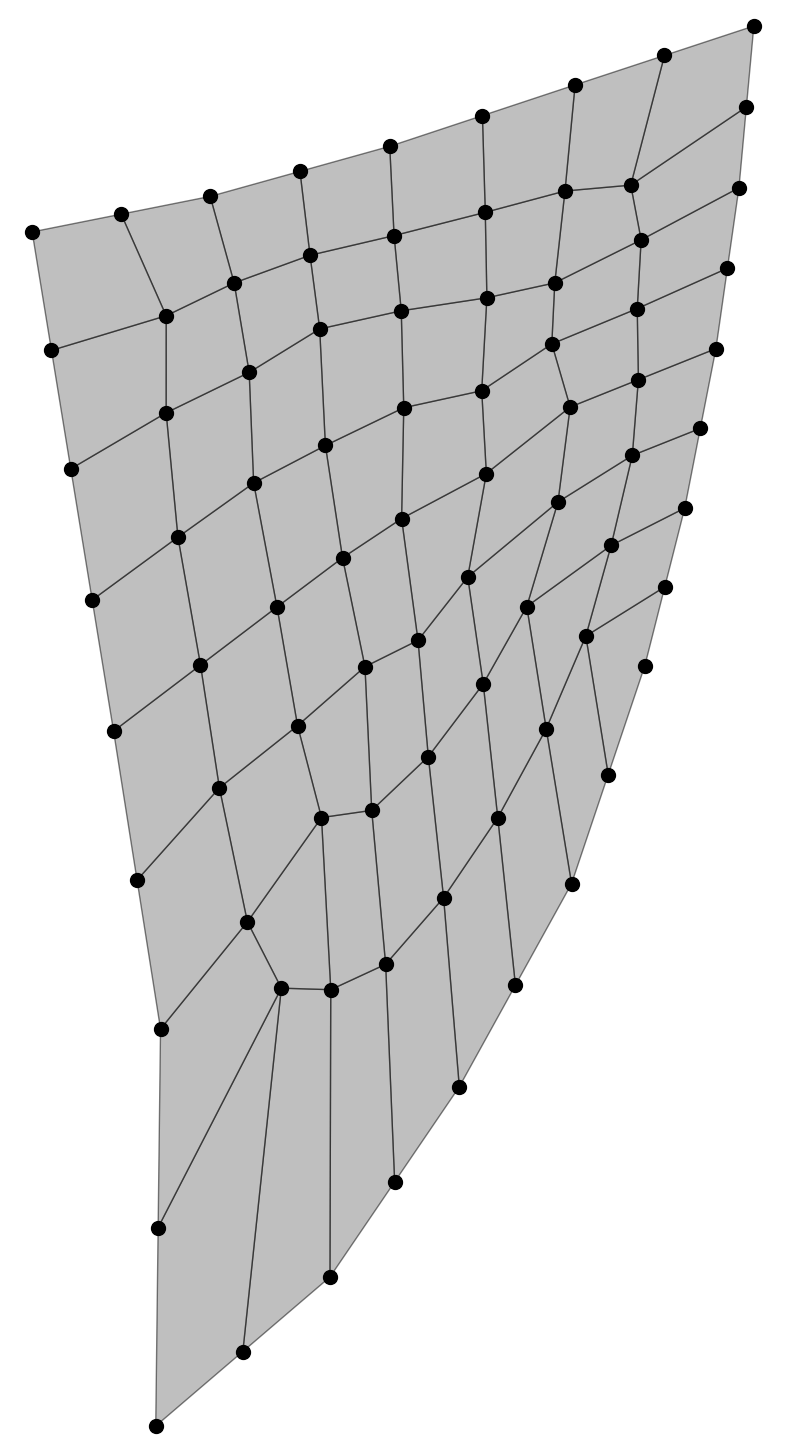
\includegraphics[height=7cm]{images/parallel_fiber_estimation/world_mesh.png}
    \caption{Initial 2D mesh of a subdomain at the border of the biceps muscle.}%
    \label{fig:world_mesh}%
  \end{subfigure}
  \quad
  \begin{subfigure}[t]{0.48\textwidth}%
    \centering%
    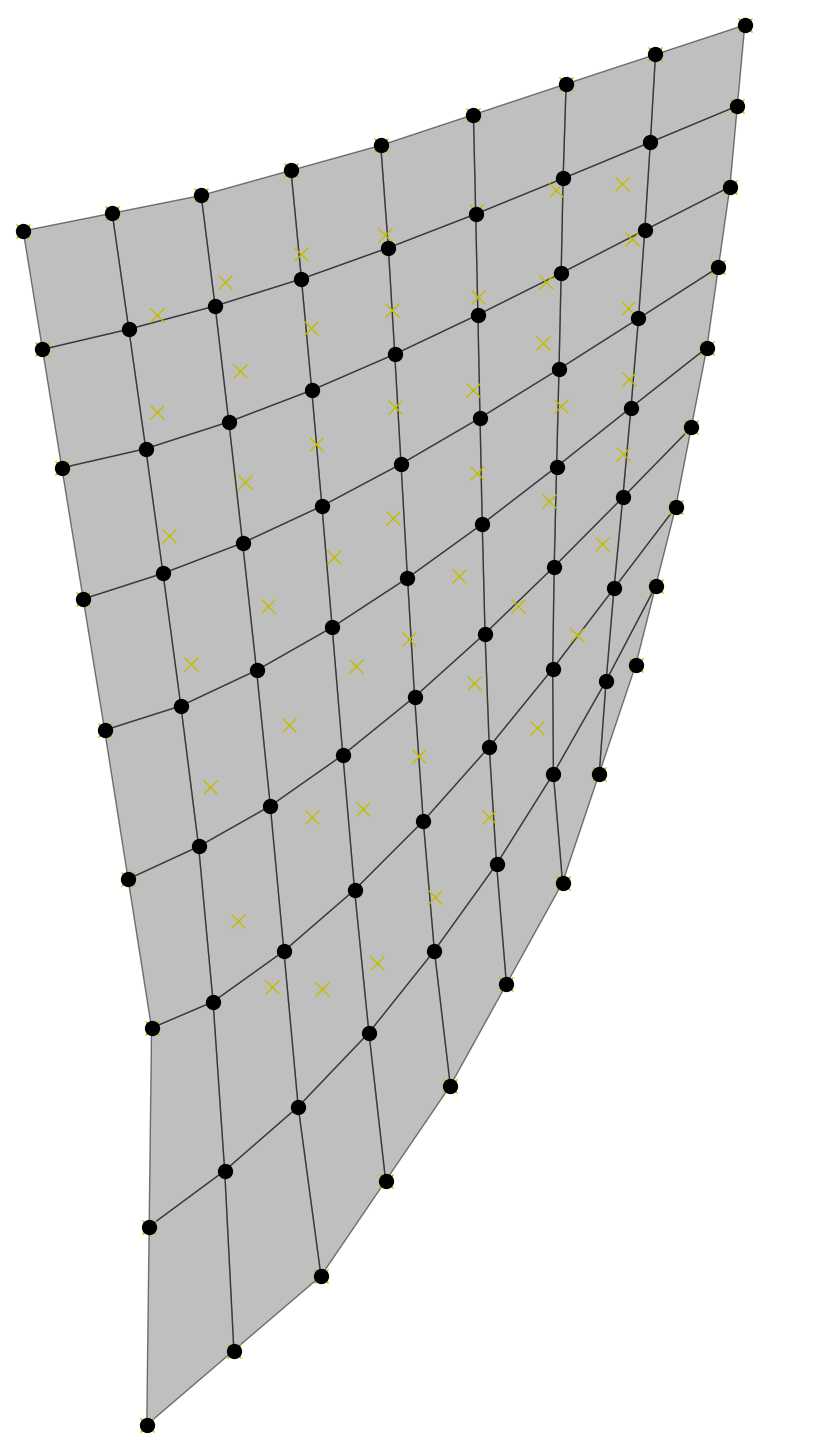
\includegraphics[height=7cm]{images/parallel_fiber_estimation/world_mesh_improved.png}
    \caption{The mesh of (\subref{fig:world_mesh}) after 20 iterations of Laplacian smoothing.}%
    \label{fig:world_mesh_improved}%
  \end{subfigure}    
  \caption{Effect of Laplacian smoothing of a 2D grid which occurs in line \algref{alg:parallel_algorithm_1}{line:3.3} of \cref{alg:parallel_algorithm_1}.}%
  \label{fig:laplace_smoothing}%
\end{figure}%

\subsection{Computation of Subdomains}

After the 3D mesh has been created and smoothened, the next steps construct the eight subdomains for the recursive calls by subdividing the own domain.
At the beginning of the procedure in \cref{alg:parallel_algorithm_1} the own domain on each process is specified by their circumferential border. More specifically, for each slice $4 \times 4$ border points are given. \Cref{fig:border_grid_1} visualizes the border points of a subdomain by the red boundary. The visualization uses a squared grid whereas in reality the domain has the shape given by (part of) the muscle cross sections. Note that a full grid with this border would contain $5 \times 5 =25 $ grid points whereas the number of considered border points is $4 \times 4 = 16$.

\begin{figure}%
  \centering%
  \begin{subfigure}[t]{0.48\textwidth}%
    \centering%
    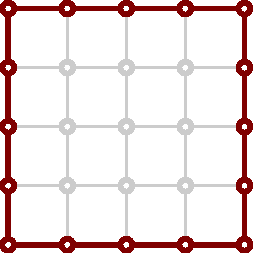
\includegraphics[width=3cm]{images/parallel_fiber_estimation/border_grid.pdf}%
   \caption{Grid of $4 \times 4$ border points, which occurs at the beginning of the procedure of \cref{alg:parallel_algorithm_1}.}%
    \label{fig:border_grid_1}%
  \end{subfigure}
  \quad
  \begin{subfigure}[t]{0.48\textwidth}%
    \centering%
    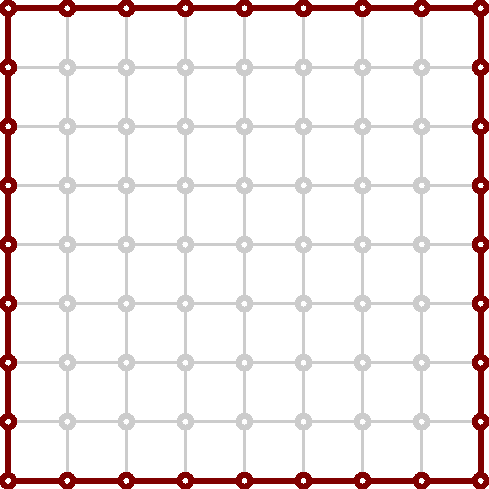
\includegraphics[width=3cm]{images/parallel_fiber_estimation/border_grid_2.pdf}%
    \caption{Grid with $4 \times 8$ border points, which occurs after a refinement step at beginning of the procedure of \cref{alg:parallel_algorithm_1}.}%
    \label{fig:border_grid_2}%
  \end{subfigure}   
  \caption{Logical grid of a subdomain (gray) specified by the border points (red) during execution of \cref{alg:parallel_algorithm_1}.}%
  \label{fig:border_grid}%
\end{figure}%

The task in the procedure is now to determine borders for eight subdomains. This is achieved by subdividing the given 2D domain into four subdomains and additionally splitting the muscle volume at the center in vertical direction.
A visualization of the resulting border points for the first and the eighth subdomain is given in \cref{fig:subdomain}.

\begin{figure}%
  \centering%
  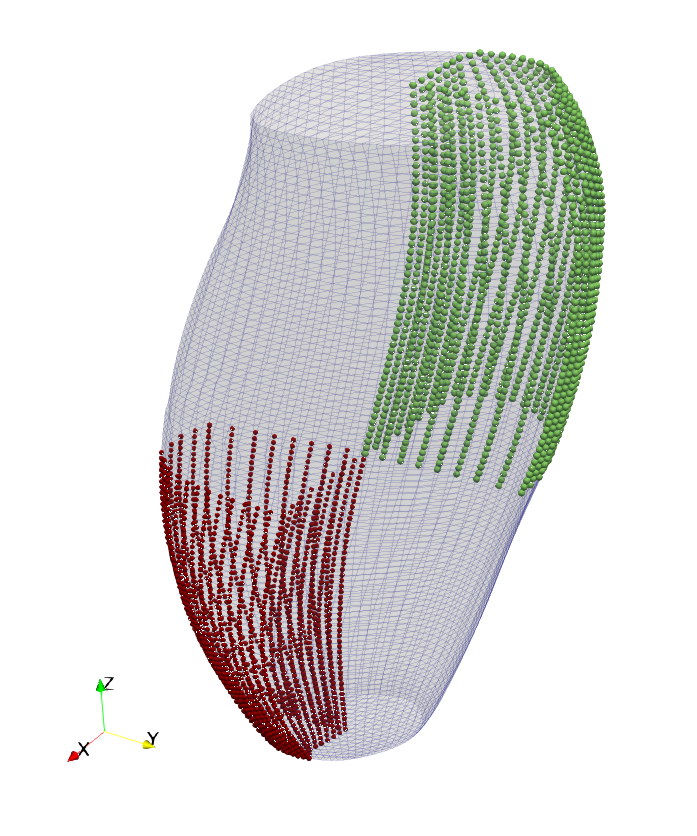
\includegraphics[height=8cm]{images/parallel_fiber_estimation/subdomains_2.png}%
  \caption{Partitioning of the muscle volume into eight subdomains during the first call to the procedure in \cref{alg:parallel_algorithm_1}. The first (red) and the eighth subdomain (green) are shown.}%
  \label{fig:subdomain}%
\end{figure}%

For this reason, the given $4 \times 4$ border points are refined to twice the amount of border points by inserting new points at the centers between neighboring points. The resulting grid is shown in \cref{fig:border_grid_2}. Now, it would be possible to subdivide the grid to obtain four instances of the needed grid in \cref{fig:border_grid_1}.
However, this would result in constant straight connection lines between the initial border points. In all further recursive calls, the additional points would all be placed on these lines and thereby not properly refine the subdomain borders. Instead, a different approach is desired where the subdomain's borders in the volume follow the directions of streamlines and fibers. Thus, the approach is to define the subdomain borders in the interior of the global domain by traced streamlines and sample the outer borders from the surface triangulation with the desired mesh width. The required steps of this approach are discussed next.

\Cref{alg:parallel_algorithm_1} proceeds with the next step in line \algref{alg:parallel_algorithm_1}{line:3.4}, which is solving the Laplace problem.
The same step also occurs in \cref{alg:serial_algorithm_2} and is explained in \cref{sec:generation_of_fiber_meshes}.
Dirichlet boundary conditions of $p(\bfx) = 0$ and $p(\bfx) = 1$ are prescribed at the bottom and top of the domain, as shown by the spheres in \cref{fig:dirichlet_bc_1}. Alternatively, Neumann boundary conditions can be used. After the solution $p(\bfx)$ is obtained, the gradient field $\nabla p(\bfx)$ is computed. The solution and the gradient directions are visualized in \cref{fig:laplace_1}.

\begin{figure}
  \centering
  \begin{subfigure}[t]{0.23\textwidth}%
    \centering%
    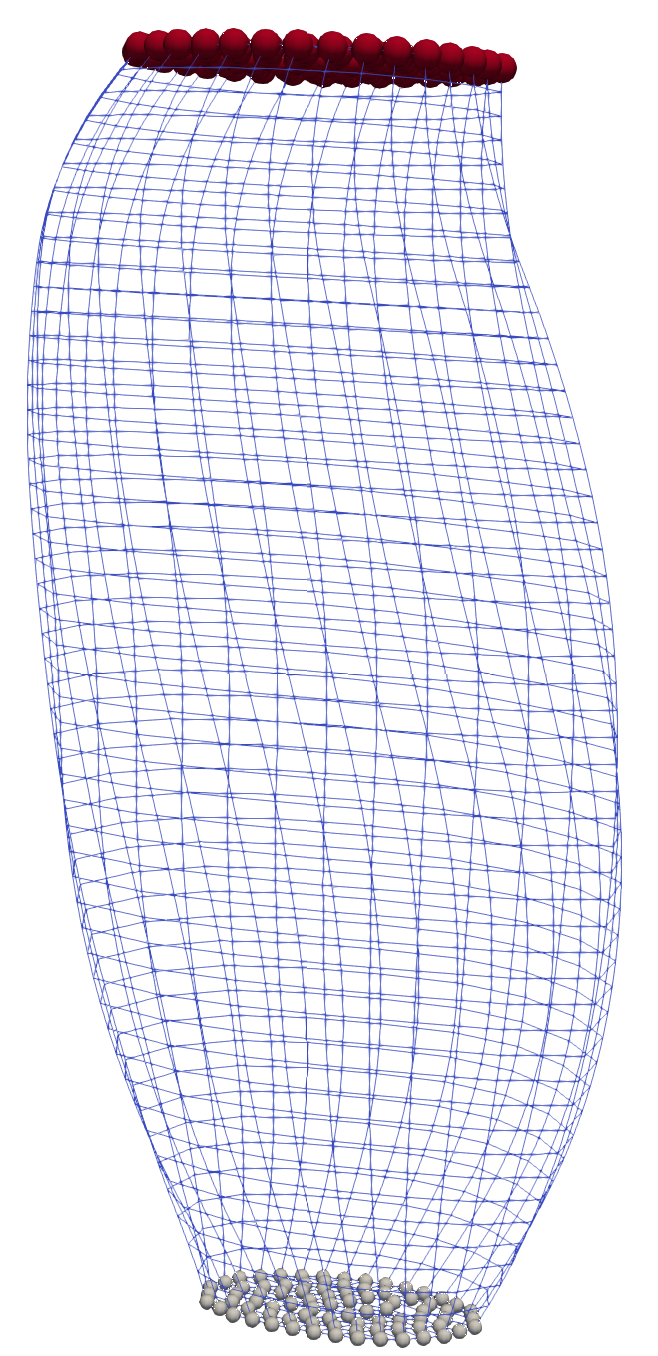
\includegraphics[height=7cm]{images/parallel_fiber_estimation/dirichlet_bc_1.png}
    \caption{Location of Dirichlet boundary condition nodes at the bottom and top.}%
    \label{fig:dirichlet_bc_1}%
  \end{subfigure}
  \,
  \begin{subfigure}[t]{0.24\textwidth}%
    \centering%
    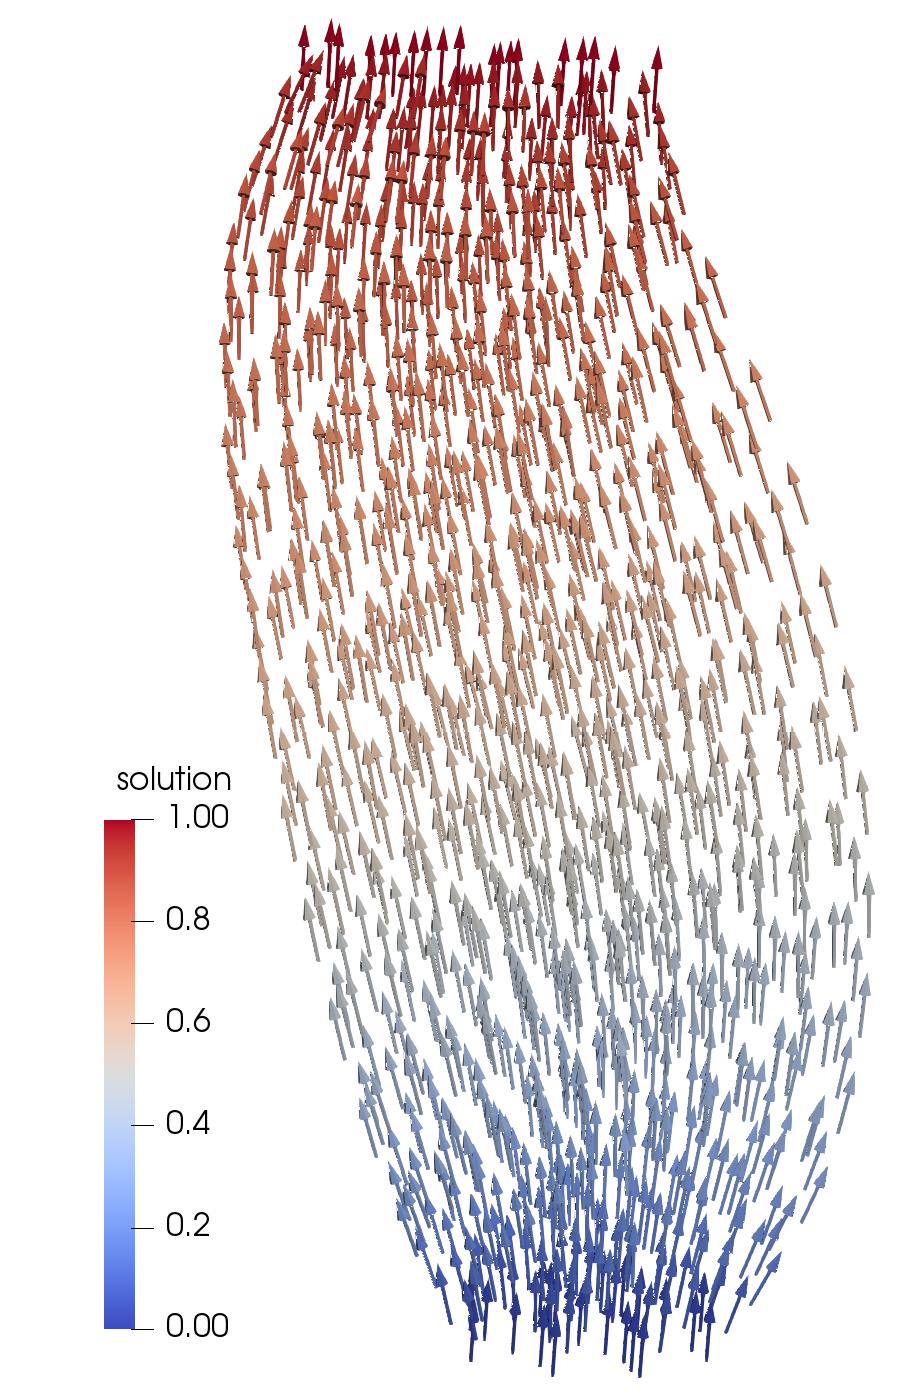
\includegraphics[height=7cm]{images/parallel_fiber_estimation/laplace_1.png}
    \caption{Solution $p$ of the Laplace problem and direction of gradient $\nabla p$.}%
    \label{fig:laplace_1}%
  \end{subfigure}
  \qquad
  \begin{subfigure}[t]{0.19\textwidth}%
    \centering%
    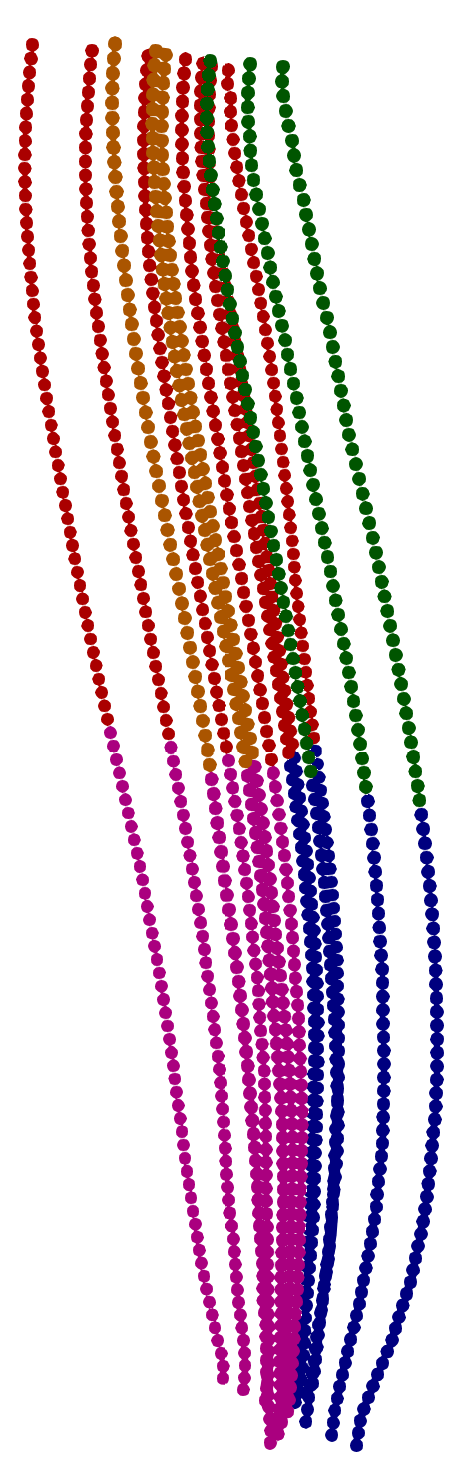
\includegraphics[height=7cm]{images/parallel_fiber_estimation/border_points_1.png}
    \caption{Traced streamlines that split the domain into eight subdomains.}%
    \label{fig:border_points_1}%
  \end{subfigure}
  \,
  \begin{subfigure}[t]{0.24\textwidth}%
    \centering%
    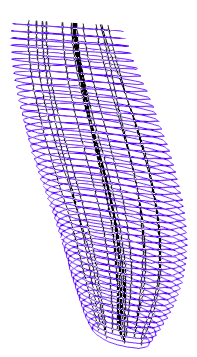
\includegraphics[height=7.2cm]{images/parallel_fiber_estimation/slices_2.png}
    \caption{Rings of the slices $S_M$ and traced streamlines in the interior.}%
    \label{fig:slices_2}%
  \end{subfigure}
  \caption{Process of subdividing the muscle volume into eight subdomains, which is an important step in the procedure of \cref{alg:parallel_algorithm_1}.}
  \label{fig:determining_subdomains}%
\end{figure}

The next step, line \algref{alg:parallel_algorithm_1}{line:3.5}, is to communicate ghost elements to neighboring subdomains. This step is only meaningful in later recursions and requires no operation in the first, serial call to the algorithm because the domain is not yet partitioned into subdomains.

Next, the algorithm traces streamlines through the gradient field in line \algref{alg:parallel_algorithm_1}{line:3.6}. This step is again similar to the analogous step in \cref{alg:serial_algorithm_2}. 
The same method of explicit Euler integration is used. 
The seed points are again chosen in the cross-sectional plane at the vertical center of the muscle. 
From there, streamlines are traced in both directions towards the ends of the muscle following the positive and negative gradient directions. In contrast to \cref{alg:serial_algorithm_2}, the horizontal locations of the seed points of the streamlines are chosen differently, because the purpose of the streamlines at this stage is not to create fiber meshes as in \cref{alg:serial_algorithm_2}.
Instead, the streamlines in \cref{alg:parallel_algorithm_1} are needed to determine the subdomain borders to partition the domain into eight subdomains. This happens in line \algref{alg:parallel_algorithm_1}{line:3.7}.

The seed points are selected from the set of nodes in the structured mesh of the 2D slice. The points selected during the first call to the procedure where the domain is not yet partitioned are shown by the red and yellow points in \cref{fig:seed_points_to_send_1}.
As can be seen, the seed points consist of the nodes of the mesh at the horizontal and vertical centers, which form a \emph{plus sign} shape. They are visualized by red points in \cref{fig:seed_points_to_send_1}.
In addition, there are four points near the corners of the structured mesh, given by the yellow points.
The border of the slice is also visualized together with a method of splitting it into eight sectors by choosing the splitting points such that they are the closest to the given outer seed points.

\begin{figure}
  \centering
  \begin{subfigure}[t]{0.30\textwidth}%
    \centering%
    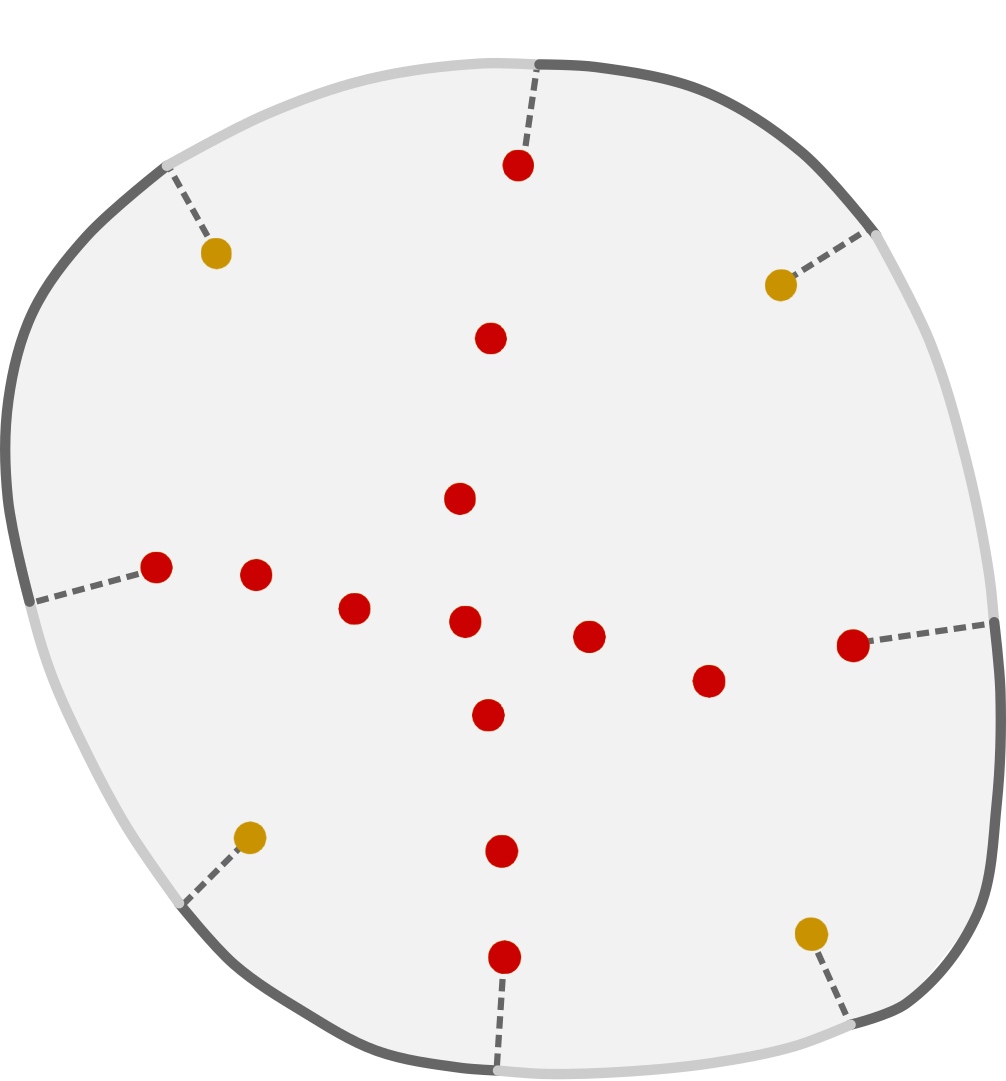
\includegraphics[height=4cm]{images/parallel_fiber_estimation/seed_points_to_send_1a.png}
    \caption{The seed points used to determine the subdomain borders. }%
    \label{fig:seed_points_to_send_1}%
  \end{subfigure}
  \,
  \begin{subfigure}[t]{0.30\textwidth}%
    \centering%
    
\includegraphics[height=4cm]{images/parallel_fiber_estimation/fixed_1.png}
    \caption{Streamlines and lines on the muscle surface that define the new subdomain borders, view from the top of the muscle.}%
    \label{fig:fixed_1}%
  \end{subfigure}
  \,
  \begin{subfigure}[t]{0.30\textwidth}%
    \centering%
    
\includegraphics[height=4cm]{images/parallel_fiber_estimation/final_interior_1.png}
    \caption{All streamlines and lines on the muscle surface that are created if the algorithm is run with one process.}%
    \label{fig:final_interior_1}%
  \end{subfigure}
  \caption{Seed points and streamlines that occur during the first call to the procedure in \cref{alg:serial_algorithm_2}.}
  \label{fig:seed_points}%
\end{figure}

The streamlines for the seed points of the plus sign are depicted in \cref{fig:border_points_1}. As shown by the different colors, these streamlines constitute the interior border points for eight subdomains that partition the muscle volume. \Cref{fig:slices_2} shows all streamlines of this first set in black and the circumferential rings of the muscle slices in blue that were extracted during the call to \cref{alg:serial_algorithm_1} in line \algref{alg:parallel_algorithm_1}{line:3.2}. 

For the new partitioning, the border points at the outer surface of the muscle are yet to be determined. For this reason, every circumferential ring needs to be split into four quarter parts for the four adjacent subdomains. For each of these new subdomains, this part corresponds to two neighboring sides of the subdomain border given in \cref{fig:border_grid_1}. Therefore, a splitting point is needed that further splits every quarter part of the circumferential ring into the two sides for the new subdomain.
In other words, the ring needs to split into eight parts that fit to the inner subdomain borders. The eight split points are determined by the eight outer streamline points. As seen in \cref{fig:seed_points_to_send_1}, the four outer red points of the plus sign and the four yellow points are considered. For each, the nearest point on the circumferential ring is determined. The algorithm for calculating the coordinates of the point on a ring that has the shortest distance to a given, second point is described in \cref{sec:slicing_of_the_geometry}.

After the two sections of the circumferential rings are determined for all new subdomains, the sections are equistantly sampled in circumferential direction to create the outer border points for the subdomains. 
Also in longitudinal direction of the muscle, i.e., the $z$ axis, points are sampled on each streamlines to yield a predefined number of points. As an example, we set the number to 51. The resulting border points are shown in \cref{fig:fixed_1}.
%The number of points in $x$ and $y$ directions is already matching the required number of $4 \times 4$ points as needed for the subdomain grid shown in \cref{fig:border_grid_1}. 
In result, one pass of the procedure in \cref{alg:parallel_algorithm_1} has created eight subdomains, that each are defined by $4 \times 4 \times 51$ border points. In the algorithm, these points are stored in the variable \emph{border\_points} that is accessed in the next recursion.

If the current recursion level $\ell$ equals the predefined maximum level $\ell_\text{max}$, the first branch of the \code{if} statement in \algref{alg:parallel_algorithm_1}{line:3.8} is taken. Then, the final 3D mesh and 1D fiber meshes are constructed. In this case, the prepared border points are not needed for a further subdivision of the domain. Instead, they are used to construct the final mesh.
In line \algref{alg:parallel_algorithm_1}{line:3.9}, additional streamlines are traced from the remaining grid points beginning at the slice at the vertical center of the muscle. \Cref{fig:final_interior_1} shows the result of this action for $l_\text{max}=1$.

Next, all streamlines are sampled at equidistant positions with a prescribed distance. The set of points forms the resulting 3D mesh of the domain $\Omega_M$. At the same time, the values can be interpreted as 1D fiber meshes $\Omega_{F,i}$, one for each traced streamline.

In the case $\ell < \ell_\text{max}$ the second branch of the \code{if} statement in \algref{alg:parallel_algorithm_1}{line:3.8} is chosen and the next recursion level $\ell_\text{new} = \ell+1$ begins. Execution continues with the eight times higher number of processes $8^{\ell_\text{new}}$.  In line \algref{alg:parallel_algorithm_1}{line:3.11a}, each process communicates its computed border points for the subdomains to the seven appropriate processes. Only the first subdomain remains on the same process. Next, in line \algref{alg:parallel_algorithm_1}{line:3.11} all now involved processes call the procedure and continue the algorithm on their own subdomains.

\subsection{Procedure on Higher Recursion Levels}
% trace streamlines from seed points, this also exchanges the seed points
% fixIncompleteStreamlines

In the following, the procedure of \cref{alg:parallel_algorithm_1} is illustrated in more detail for higher recursion levels, where multiple processes concurrently work on their own subdomain. The input consists of the given $4 \times 4 \times 51$ border points for the local subdomain of the process, which, as mentioned, get initially refined to $8 \times 8 \times 51$ border points. \Cref{fig:subdomain} shows the refined border points for the subdomain of the first process in recursion level $\ell=1$ in red. This subdomain will be considered in the following examples.

To obtain a sufficiently fine 3D mesh, the 2D mesh gets refined further by increasing the number of elements per coordinate direction by a factor of $r\in \N$. For example, $r=2$ refines the grid to $16 \times 16$ border points on each slice. This is shown in \cref{fig:02_border_points} in a view in negative $z$ direction. The red points are the border points of the $9 \times 9$ grid, the additional white points are added in between. At the lower left of the figure, it can be seen that always five neighboring points lie on a straight line since the initial border points were refined two times by taking center points between existing points. The border points on the curved outer boundary were instead sampled from the surface triangulation and do not show this behavior.

In line \algref{alg:parallel_algorithm_1}{line:3.2} of \cref{alg:parallel_algorithm_1}, the harmonic mesh algorithm to construct a 3D mesh, \cref{alg:serial_algorithm_1}, is called. Its input consists of the points shown in \cref{fig:02_border_points}, which define the 2D slices of the volume. This means that the \cref{alg:serial_algorithm_1} does not need to construct the slice border rings from the surface triangulation, instead, the formulation of \cref{alg:serial_algorithm_1} can directly start with line \algref{alg:serial_algorithm_1}{alg:1.2} to triangulate the slices and then compute the harmonic map.


In line \algref{alg:parallel_algorithm_1}{line:3.4} of \cref{alg:parallel_algorithm_1}, the Laplace problem gets solved. The equation is formulated globally and the discretization uses the existing partitioning. The system matrix is indefinite if Dirichlet boundary conditions are used. A parallel GMRES solver obtains the solution in a small number of iterations, e.g., for the biceps muscle that yields a linear system with 4131 degrees of freedom, 26 iterations are needed to obtain a residual norm of below \num{1e-4}.

Next, the seed points for the streamlines are determined. \Cref{fig:03_seed_points} shows the seed points in blue. In addition to the plus sign shape and the four outer seed points, two lines of points in approximate $x$ and $y$ directions are selected at the lower and right edges of the figure. These are needed to determine the outer borders of the new subdomains that lie in the interior of the muscle. Thus, the existing subdomain borders inside the muscle are recreated using streamlines. The streamlines are traced in the gradient field of the solution of the Laplace problem that is solved on the finer mesh. In general, such lines of seed points are required on any border of the subdomain, whenever the border is in the interior of the muscle.

\begin{figure}%
  \centering%
  \begin{subfigure}[t]{0.45\textwidth}%
    \centering%
    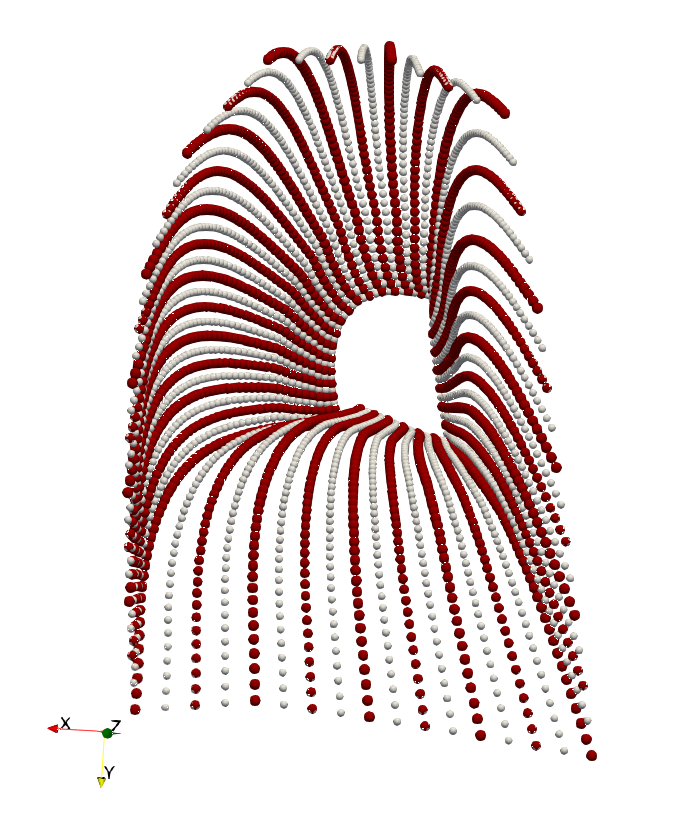
\includegraphics[height=9cm]{images/parallel_fiber_estimation/02_border_points_2.png}
    \caption{Refined border points.}%
    \label{fig:02_border_points}%
  \end{subfigure}   
  \quad
  \begin{subfigure}[t]{0.45\textwidth}%
    \centering%
    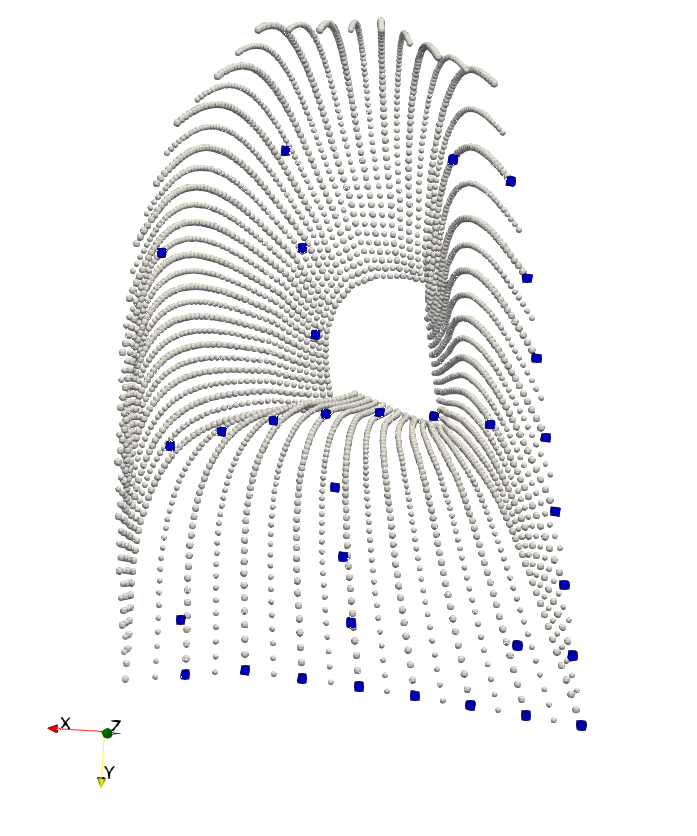
\includegraphics[height=9cm]{images/parallel_fiber_estimation/03_seed_points.png}
    \caption{Seed points for the streamlines.}%
    \label{fig:03_seed_points}%
  \end{subfigure}
  \\
  \begin{subfigure}[t]{0.45\textwidth}%
    \centering%
    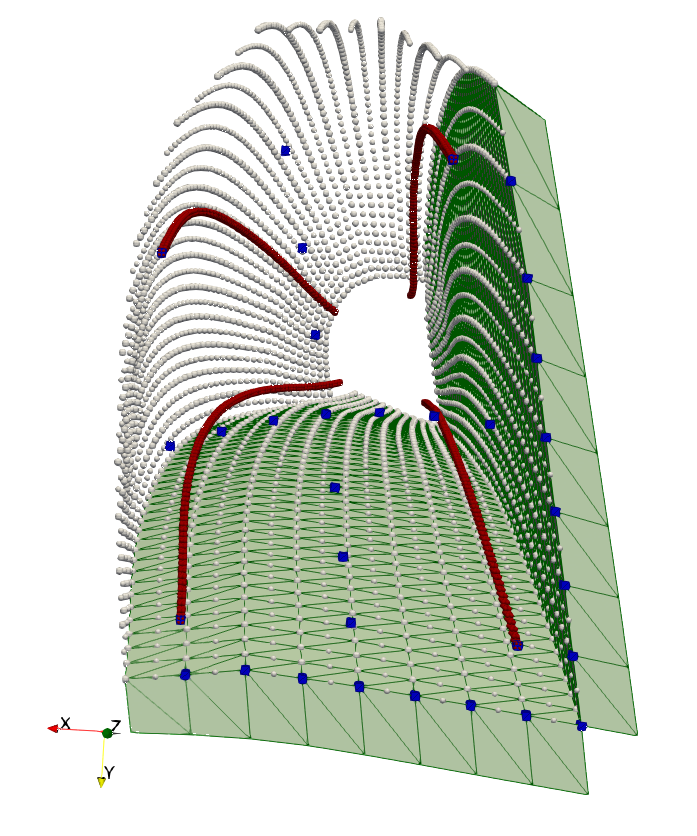
\includegraphics[height=8cm]{images/parallel_fiber_estimation/05_corner_streamlines.png}
    \caption{The four border streamlines (red) and the green layers of ghost elements at the bottom and right of the subdomain.}%
    \label{fig:05_corner_streamlines}%
  \end{subfigure}   
  \quad
  \begin{subfigure}[t]{0.45\textwidth}%
    \centering%
    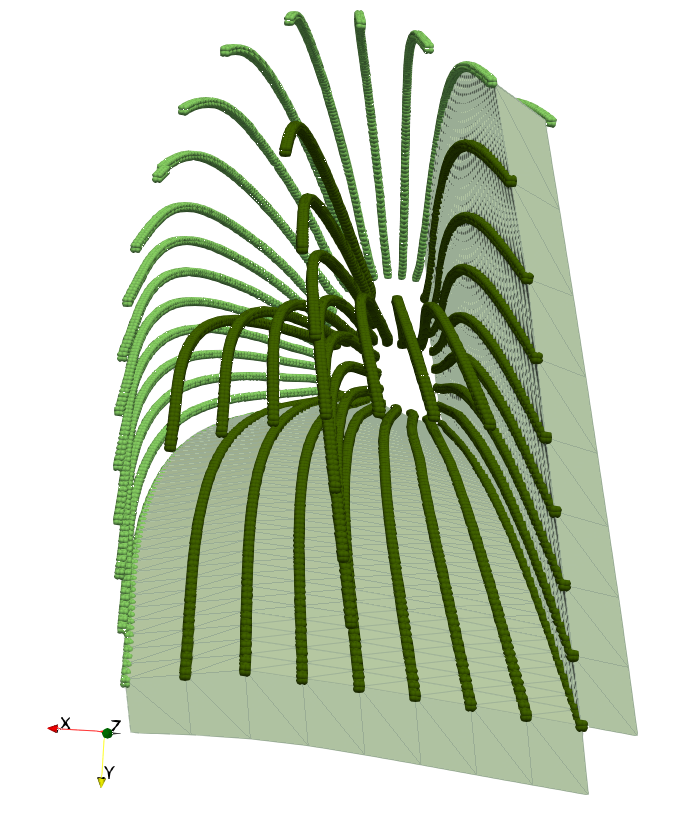
\includegraphics[height=8cm]{images/parallel_fiber_estimation/07_filled.png}
    \caption{New border points at the outer (light green) and interior border (dark green).}%
    \label{fig:07_filled}%
  \end{subfigure}  
  \caption{Streamlines in the first subdomain for recursion level $l=1$ of the parallel algorithm for mesh generation.}%
  \label{fig:03_border_points_and_seed_points}%
\end{figure}%

Tracing those interior border streamlines using only the locally stored data of the subdomain usually fails. These streamlines start exactly on the border of the subdomain and potentially leave the local subdomain by a small distance because to the solution on the finer mesh is slightly different than the solution on the previous, coarser mesh. To account for this effect, the solution data from the neighboring 3D mesh elements is needed at those locations. For this reason, the algorithm communicates one layer of \emph{ghost elements} between neighboring processes such that every subdomain knows the adjacent elements at the interior borders. This occurs in line \algref{alg:parallel_algorithm_1}{line:3.5} of the algorithm and involves communicating the node positions and the values of the gradient field between the respective processes. \Cref{fig:05_corner_streamlines} shows the received ghost elements on the considered subdomain in green.


The next step is to trace the streamlines in line \algref{alg:parallel_algorithm_1}{line:3.6} of the algorithm. Since the streamlines traverse the entire muscle from the center to bottom and top, this step involves multiple processes. All processes are numbered in $z$ direction from bottom to top by an index $i_z \in \{0, 1, \dots, n_z-1\}$ where the number of processes in $z$ direction is $n_z = 2^\ell$.

The initial seed points are determined on the processes with index $\lfloor n_z/2\rfloor$. They are communicated to the processes below with index $\lfloor n_z/2\rfloor-1$. Then, these two groups of processes  trace the streamlines starting from the same seed points through their subdomains, the upper processes in upward and the lower processes in downward direction. Then, the end points of the traced fibers are communicated to the next processes which continue the tracing of the streamlines. The procedure repeats with further processes until the streamlines reach the bottom and top ends of the overall muscle domain.
The time complexity of this approach is $\O(n_z) = \O(\sqrt[3]{n_\text{proc}})$ with the number $n_\text{proc}$ of processes.

The tracing algorithm in the subdomains uses the efficient scheme of predicting subsequently traversed elements described in \cref{sec:algorithm_for_streamline_tracing}. The implementation is adjusted in a way to also take into account the ghost elements.

The red streamlines in \cref{fig:05_corner_streamlines} are the ones to split the border sides at the outer boundary of the global domain. For simplicity, the algorithm always computes the four streamlines in every corner of the mesh. In the considered example, only the streamline in the upper left corner is needed to sample the border points. \Cref{fig:07_filled} shows the sampled border points at the surface in light green color. The two sides of the own domain will be split into four sides for the new subdomains, therefore the surface gets sampled at $4\times 4=16$ lines. A comparison with the white lines in \cref{fig:05_corner_streamlines} shows that the newly sampled points are different from the initially sampled points. 

\Cref{fig:07_filled} visualizes the traced streamlines in the interior with dark green color. They are used as border points for the eight new subdomains. The border of the first of the new subdomains on level $l=2$ is shown in \cref{fig:06_subdomain}. It consists of the outer border (dark yellow lines) and the interior border (brown streamlines) and is nearly geometrically similar to the subdomain on level $l=1$. 

If the recursion ends at level $\ell=1$, the algorithm creates 3D and 1D meshes instead of new subdomains. Then, streamlines are traced for all grid points of the current subdomain mesh. \Cref{fig:08_final} visualizes the seed points and the traced streamlines in this case. In the parallel setting, this action is organized analogous to the previous tracing of streamlines: The tracing starts at the vertical center of the muscle and subsequently propagates through all layers of subdomains in $z$ direction. 

At the end, the data is written collectively by all processes into a single file. This is done using the parallel file I/O functionality of MPI. It is possible because the absolute position in the file of every point can be calculated from the index of the point in the structured mesh.


\begin{figure}%
  \centering%
  \begin{subfigure}[t]{0.45\textwidth}%
    \centering%
    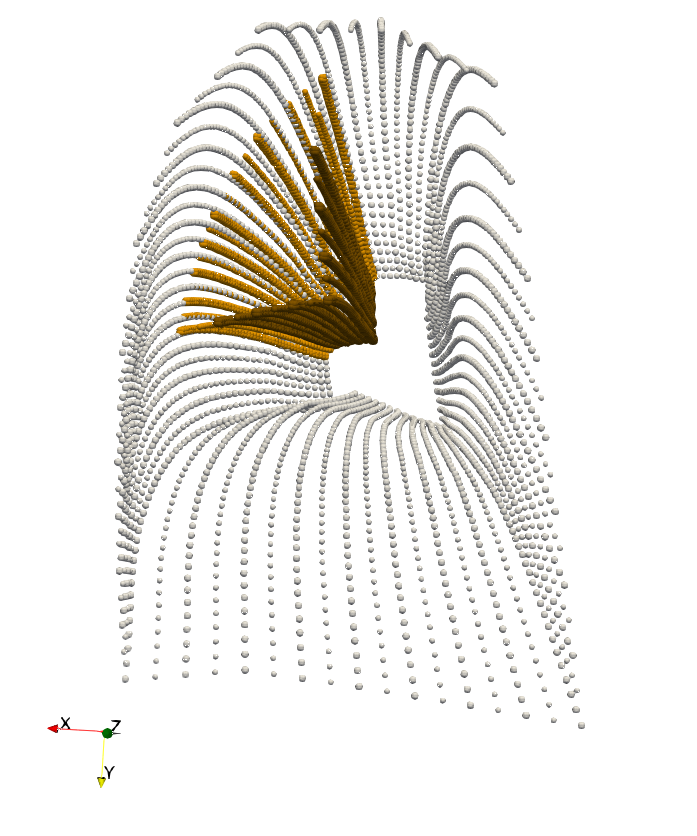
\includegraphics[height=8cm]{images/parallel_fiber_estimation/06_subdomain.png}
    \caption{Border points of the first subdomain on level $l=2$ (dark yellow and brown) embedded in the border (white) of level $l=1$, generated if $l_\text{max} > 1$.}%
    \label{fig:06_subdomain}%
  \end{subfigure}
  \quad
  \begin{subfigure}[t]{0.45\textwidth}%
    \centering%
    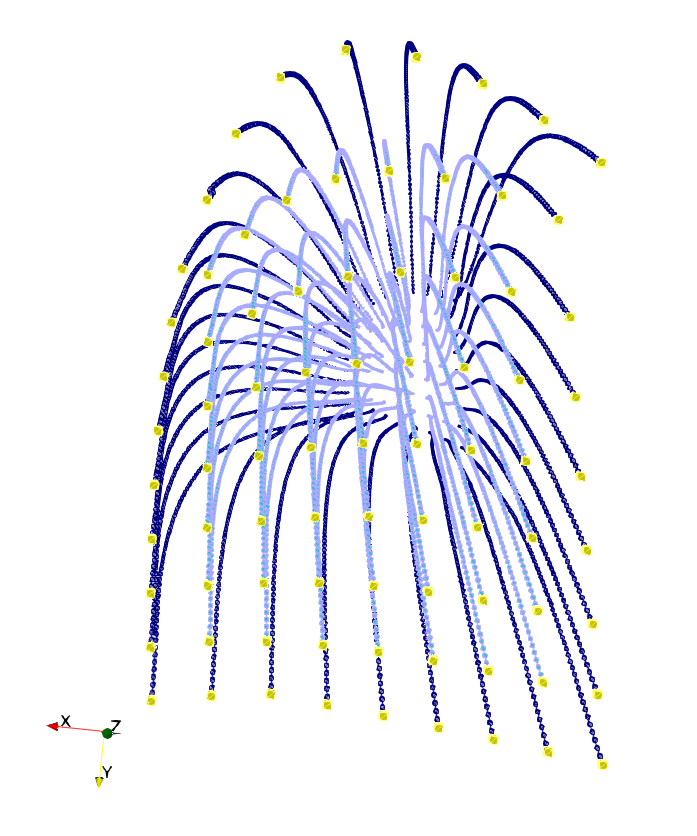
\includegraphics[height=8cm]{images/parallel_fiber_estimation/08_final.png}
    \caption{Seed points (yellow), traced interior streamlines (light blue) and border points (dark blue), generated if $l_\text{max}=1$.}%
    \label{fig:08_final}%
  \end{subfigure}   
   
  \caption{Results of the procedure in the parallel algorithm for mesh generation.}%
  \label{fig:improved}%
\end{figure}%

\subsection{Repair of Incomplete Streamlines}

Practical tests have shown that for irregular muscle geometries some of the streamlines generated in lines \algref{alg:parallel_algorithm_1}{line:3.6} and \algref{alg:parallel_algorithm_1}{line:3.9} of the algorithm are incomplete. This means that it was not possible to obtain a streamline that runs through the entire subdomain or the entire muscle domain from top to bottom, instead points are missing for some ranges of $z$ values. This happens when the streamlines run out of the subdomain.

To fix these cases, four different repair mechanisms are introduced that interpolate the missing data from valid streamlines. \Cref{fig:fix_invalid} visualizes the cases by examples in a setting of four subdomains with grids of $5 \times 5$ fibers each. The repair mechanisms $\#1$ to $\#3$ only apply to border points. They are executed in line \algref{alg:parallel_algorithm_1}{line:3.6} of the algorithm after the local portions of the streamlines have been traced and before the end points of the streamlines are sent to the neighbor processes below and above that continue the streamline tracing. Mechanism $\#4$ repairs invalid streamlines in the final result and is executed during line \algref{alg:parallel_algorithm_1}{line:3.9}.

Mechanism \#1 checks all streamlines at borders in the interior, which are shared between neighboring processes. If a streamline is incomplete on one process but complete on the neighbor process, the complete data is transferred such that both processes have the same valid points for this streamline. In the example in \cref{fig:fix_invalid}, the valid streamline data is sent from the top left to the top right subdomain.

Mechanism \#2 checks streamlines at the outer corners of the subdomains. Incomplete streamlines at these locations are recreated from the given border points. Because the set of border points is twice as coarse as the required number of sampled points at these streamlines, every second point gets interpolated from the top and bottom neighbor points.

Mechanism \#3 is concerned with streamlines at interior borders that could not be fixed by mechanism \#1 because the streamlines are incomplete on both sharing processes. In this case, the streamlines are interpolated from the two complete neighboring streamlines that are located next along the border as shown in the example in \cref{fig:fix_invalid}. Instead of the factors $\frac13$ and $2\frac23$, the actual relation of distances between the seed points of the streamlines is used. The same interpolation is executed independently on both involved processes. Because the valid streamlines have the same data on both subdomains the resulting fixed streamlines will also be identical.

Mechanism \#4 follows a similar approach. It is applied to the interior fibers of the final result and can repair any number of incomplete fibers that are located between complete fibers. In the example \#4a in \cref{fig:fix_invalid}, the two invalid streamlines are interpolated from their left and right valid neighbors. In the example \#4b, no valid right neighbor exists. Instead, the streamlines are interpolated by using valid positions from the upper and lower neighbors.

\begin{figure}%
  \centering%
  \def\svgwidth{0.8\textwidth}
  \input{images/parallel_fiber_estimation/fix_invalid.pdf_tex}
  \caption{Examples of the four repair mechanisms for estimating incomplete streamlines during the parallel algorithm for mesh generation. Invalid streamlines are indicated by red circles, valid streamlines by black circles. The brown arrows show the direction of data transfer.}%
  \label{fig:fix_invalid}%
\end{figure}%

\subsection{Postprocessing of the Generated Streamlines}

After repairing invalid streamlines, the final result of the algorithm is a grid with $(8\,n_x+1) \times (8\,n_x+1)$ fibers in the $x$-$y$ plane and a configurable number of points in $z$ direction, where $n_x = 2^{\ell_\text{max}}$ is the number of subdomains per coordinate direction on the last recursion level. 

If a higher number of fibers is desired than is naturally generated by the parallel algorithm, additional fibers can be created by interpolation in the existing grid of fibers. The implementation of the presented algorithm in \opendihu{} includes this postprocessing functionality as part of the mesh generation program. Alternatively, the step can be applied separately on any binary output file that contains a grid of fibers. 

The action of increasing the number of fibers proceeds as follows. The initial grid contains the fibers that were created from the streamlines, called \emph{key fibers}.
A specified number $m$ of additional fibers is placed evenly between the key fibers in both $x$ and $y$ coordinate directions.
The additional fibers together with the key fibers form a grid of fibers in the muscle cross sections with an $m$ times finer mesh width. In the grid of key fibers, every portion bounded by $2 \times 2$ key fibers contains $(2+m)^2 - 4$ additional fine fibers. The total number of fibers depending on $n_x$ and $m$ therefore is $N=(8\,n_x\,(1+m)+1)^2$. Due to construction of the algorithm, this number is always odd. This is a desired property because it yields an even number of elements per coordinate direction and this allows to construct a mesh with quadratic elements.

The new fibers are computed by barycentric interpolation. The location of every new point $\bfp$ is calculated from the nearest points $\bfp_0, \bfp_1, \bfp_2$ and $\bfp_3$ of key fibers in the $x$-$y$ plane, numbered according to  \cref{fig:quads_tris}, by%
\begin{align*}
  \bfp = (1-\alpha_x)\,(1-\alpha_y)\,\bfp_0 + \alpha_x\,(1-\alpha_y)\,\bfp_1 
        + (1-\alpha_x)\,\alpha_y\,\bfp_2 + \alpha_x\,\alpha_y\,\bfp_3.
\end{align*}
Here, the factors $\alpha_x,\alpha_y \in [0,1]$ are chosen in a way to create the fine grid of fibers:
%
\begin{align*}
  \alpha_x = i / (m+1), \quad \alpha_y = j / (m+1)\quad \text{ for }i,j = 0, \dots,m, \quad (i,j) \neq (0,0).
\end{align*}
In result, we can generate a 3D mesh where the number of points in $x$ and $y$ direction can be adjusted by the parameter $m$.

The points are stored in a binary file format. The contents of this output file can be either interpreted as grid points of a 3D mesh or as points of individual fibers. This is an advantage in a multi-scale simulation where both a 3D muscle mesh and multiple embedded 1D fiber meshes occur: First, all mesh information of both $\Omega_M$ and $\Omega_{F,i}$ can be given by a single file. And second, the 3D mesh is aligned with the 1D fibers and all 3D mesh points are also 1D mesh points. 

The spacing in $z$ direction between points on a fiber is chosen as $\Delta z = \SI{0.01}{\cm}$. This value was found to ensures a low error in the model for propagation of electric stimuli along the muscle. The value leads to 1481 points per fiber on the belly of the biceps muscle. Every point coordinate is stored in the output file as double precision value with \SI{8}{\byte}. The file contains a header of \SI{72}{\byte} with descriptive information such as the number of fibers, some parameter values and a time stamp. The total file size therefore can be calculated by $72+N\cdot 1481\cdot 3\cdot \SI{8}{\byte}$.

Often, the spatial resolution of the 3D mesh does not need to be as high as those of the fibers. In such a case, the 3D mesh can be constructed by only using a subset of the points given in the file. A stride in $x$, $y$ and $z$ direction is used to sample points for the structured 3D mesh.
%The 1D fiber meshes use all given points in the file.
% When a 3D mesh with a smaller spatial resolution in $x$ and $y$ direction than the number of fibers is used in a simulation together with 1D fiber meshes from the same file, some of the fibers at the outer layer can be located outside of the 3D mesh. A way to avoid this is to not use the outer layer of fibers. 


A remaining issue concerns the mesh quality on the outer border. In general, the 3D mesh created by \cref{alg:parallel_algorithm_1} has good quality because the interior points result from smooth streamlines that were traced through a divergence free vector field. 
The points at the border, however, are sampled from a triangulation of a tubular surface of the muscle. This surface is derived from imaging data, as described in \cref{sec:preprocessing_of_the_muscle_geometry}. Therefore, the quality of the border points of the created mesh depends on the quality of the muscle surface and its triangulation. In a case where this quality is poor, only the outer layer of elements of the created 3D mesh is affected. \Cref{fig:poor_border_33x33} shows an example for this effect in a grid of $9 \times 9$ fibers. It can be seen that only the fibers at the bottom of the image have an irregularity at their center. Such an irregularity potentially occurs at every $z$ coordinates where a new subdomain begins. The cause is that the points on the rings are slightly shifted relative to each other.

A remedy in such a case is to discard the outer layer of fibers and construct the mesh only from points of the inner streamlines.
Accordingly, the implementation of the presented algorithm \cref{alg:parallel_algorithm_1} always creates two different output files. The first output file contains all fibers, the second contains all except the outer layer of fibers. The second file contains only $N=(8\,n_x\,(1+m)-1)^2$ instead of $N=(8\,n_x\,(1+m)+1)^2$ fibers.
\begin{figure}%
  \centering%
  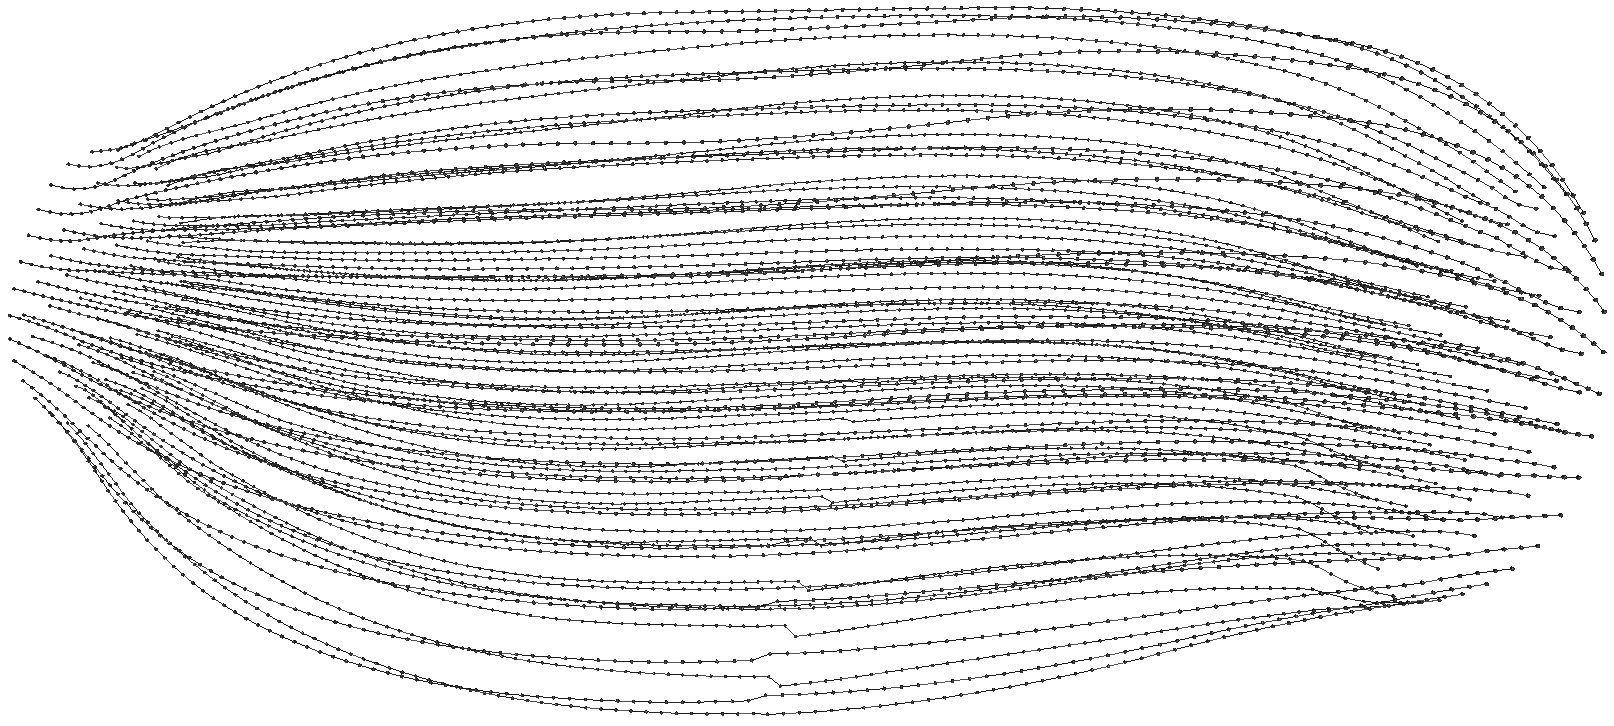
\includegraphics[width=\textwidth]{images/parallel_fiber_estimation/poor_border_33x33.png}%
  \caption{Resulting fibers and points on the fibers created with the parallel algorithm, $9\times 9$ fibers with $1481$ nodes each. Irregularities in the outer surface can be seen in the  center at the bottom if the image.}%
  \label{fig:poor_border_33x33}%
\end{figure}%

\subsection{Results and Discussion}

In the following section, meshes that were generated by \cref{alg:parallel_algorithm_1} are shown and the influence of various parameters is discussed.
\Cref{fig:muscle_meshes} visualizes some results for the biceps and triceps muscles. If the recursion level is set to $l_\text{max}=0$, the algorithm generates meshes with the smallest possible number of fibers, which is a grid of $7 \times 7$ fibers.  
\Cref{fig:muscle_mesh_0} shows a grid of $7\times 7$ fibers and the corresponding 3D mesh that was sampled from the fiber data using every 50th point in $z$ direction of the fiber meshes. It can be seen that the generated fibers traverse all nodes of the generated 3D mesh and, thus, the 3D mesh is aligned with the fiber direction.

\Cref{fig:muscle_mesh_1} shows a similar result with $9 \times 9$ fibers. Here, the colors correspond to the solution of an electrophysiology simulation. Blue regions indicate that the fiber membranes have an electric potential equal to their resting potential, which indicates no activation. Orange and red colors correspond to activated regions. It can be seen that the activation is present at the same locations on both the fibers and the 3D mesh. In the simulation, this requires data mapping from the fiber meshes to the 3D mesh. Because all nodes of the 3D mesh are located on the fibers, this data transfer becomes trivial.

\Cref{fig:muscle_mesh_2,fig:muscle_mesh_3} present grids with $13 \times 13$ and $67 \times 67$ fibers of the biceps muscle, respectively. Results with larger numbers of fibers are not shown here because in such visualizations the fibers become less distinguishable. \Cref{fig:muscle_mesh_4,fig:muscle_mesh_5} show fibers for the triceps geometry.

\begin{figure}%
  \centering%
  \begin{subfigure}[t]{0.30\textwidth}%
    \centering%
    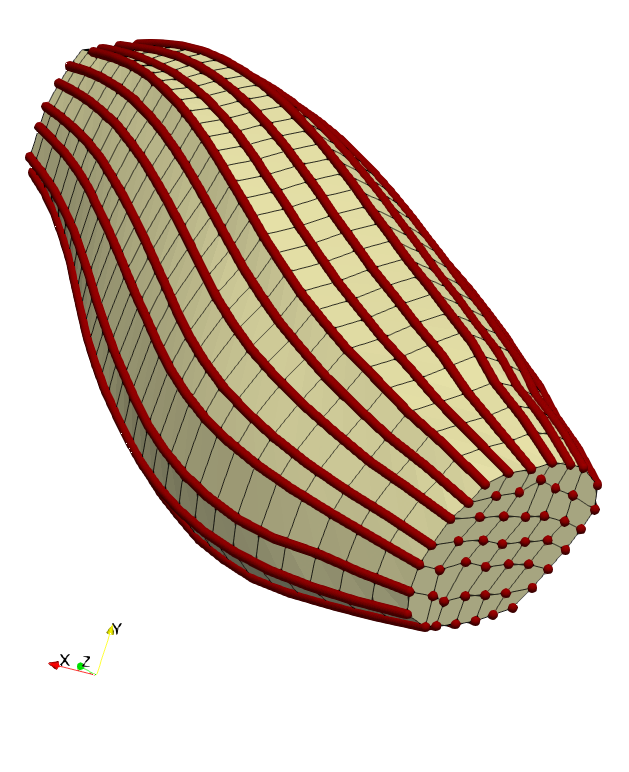
\includegraphics[height=7cm]{images/parallel_fiber_estimation/muscle_mesh.png}
    \caption{Grid of $7 \times 7$ fibers (red) and the aligned 3D mesh with $7 \times 7 \times 30$ nodes (yellow).}%
    \label{fig:muscle_mesh_0}%
  \end{subfigure}
  \quad
  \begin{subfigure}[t]{0.30\textwidth}%
    \centering%
    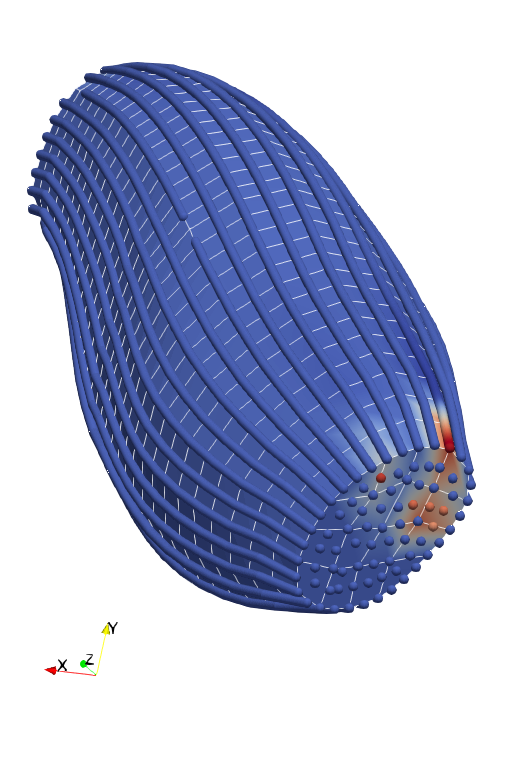
\includegraphics[height=7cm]{images/parallel_fiber_estimation/muscle_mesh_1b.png}
    \caption{Grid of $9 \times 9$ fibers and 3D mesh with the solution of an electrophysiology simulation.}%
    \label{fig:muscle_mesh_1}%
  \end{subfigure}  
  \quad 
  \begin{subfigure}[t]{0.30\textwidth}%
    \centering%
    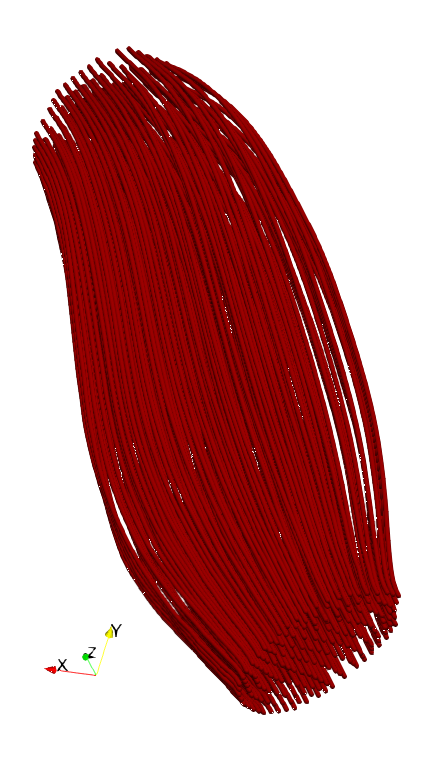
\includegraphics[height=7cm]{images/parallel_fiber_estimation/muscle_mesh_2b.png}
    \caption{Grid of $13 \times 13$ fibers.}%
    \label{fig:muscle_mesh_2}%
  \end{subfigure}
  \\
  \begin{subfigure}[t]{0.25\textwidth}%
    \centering%
    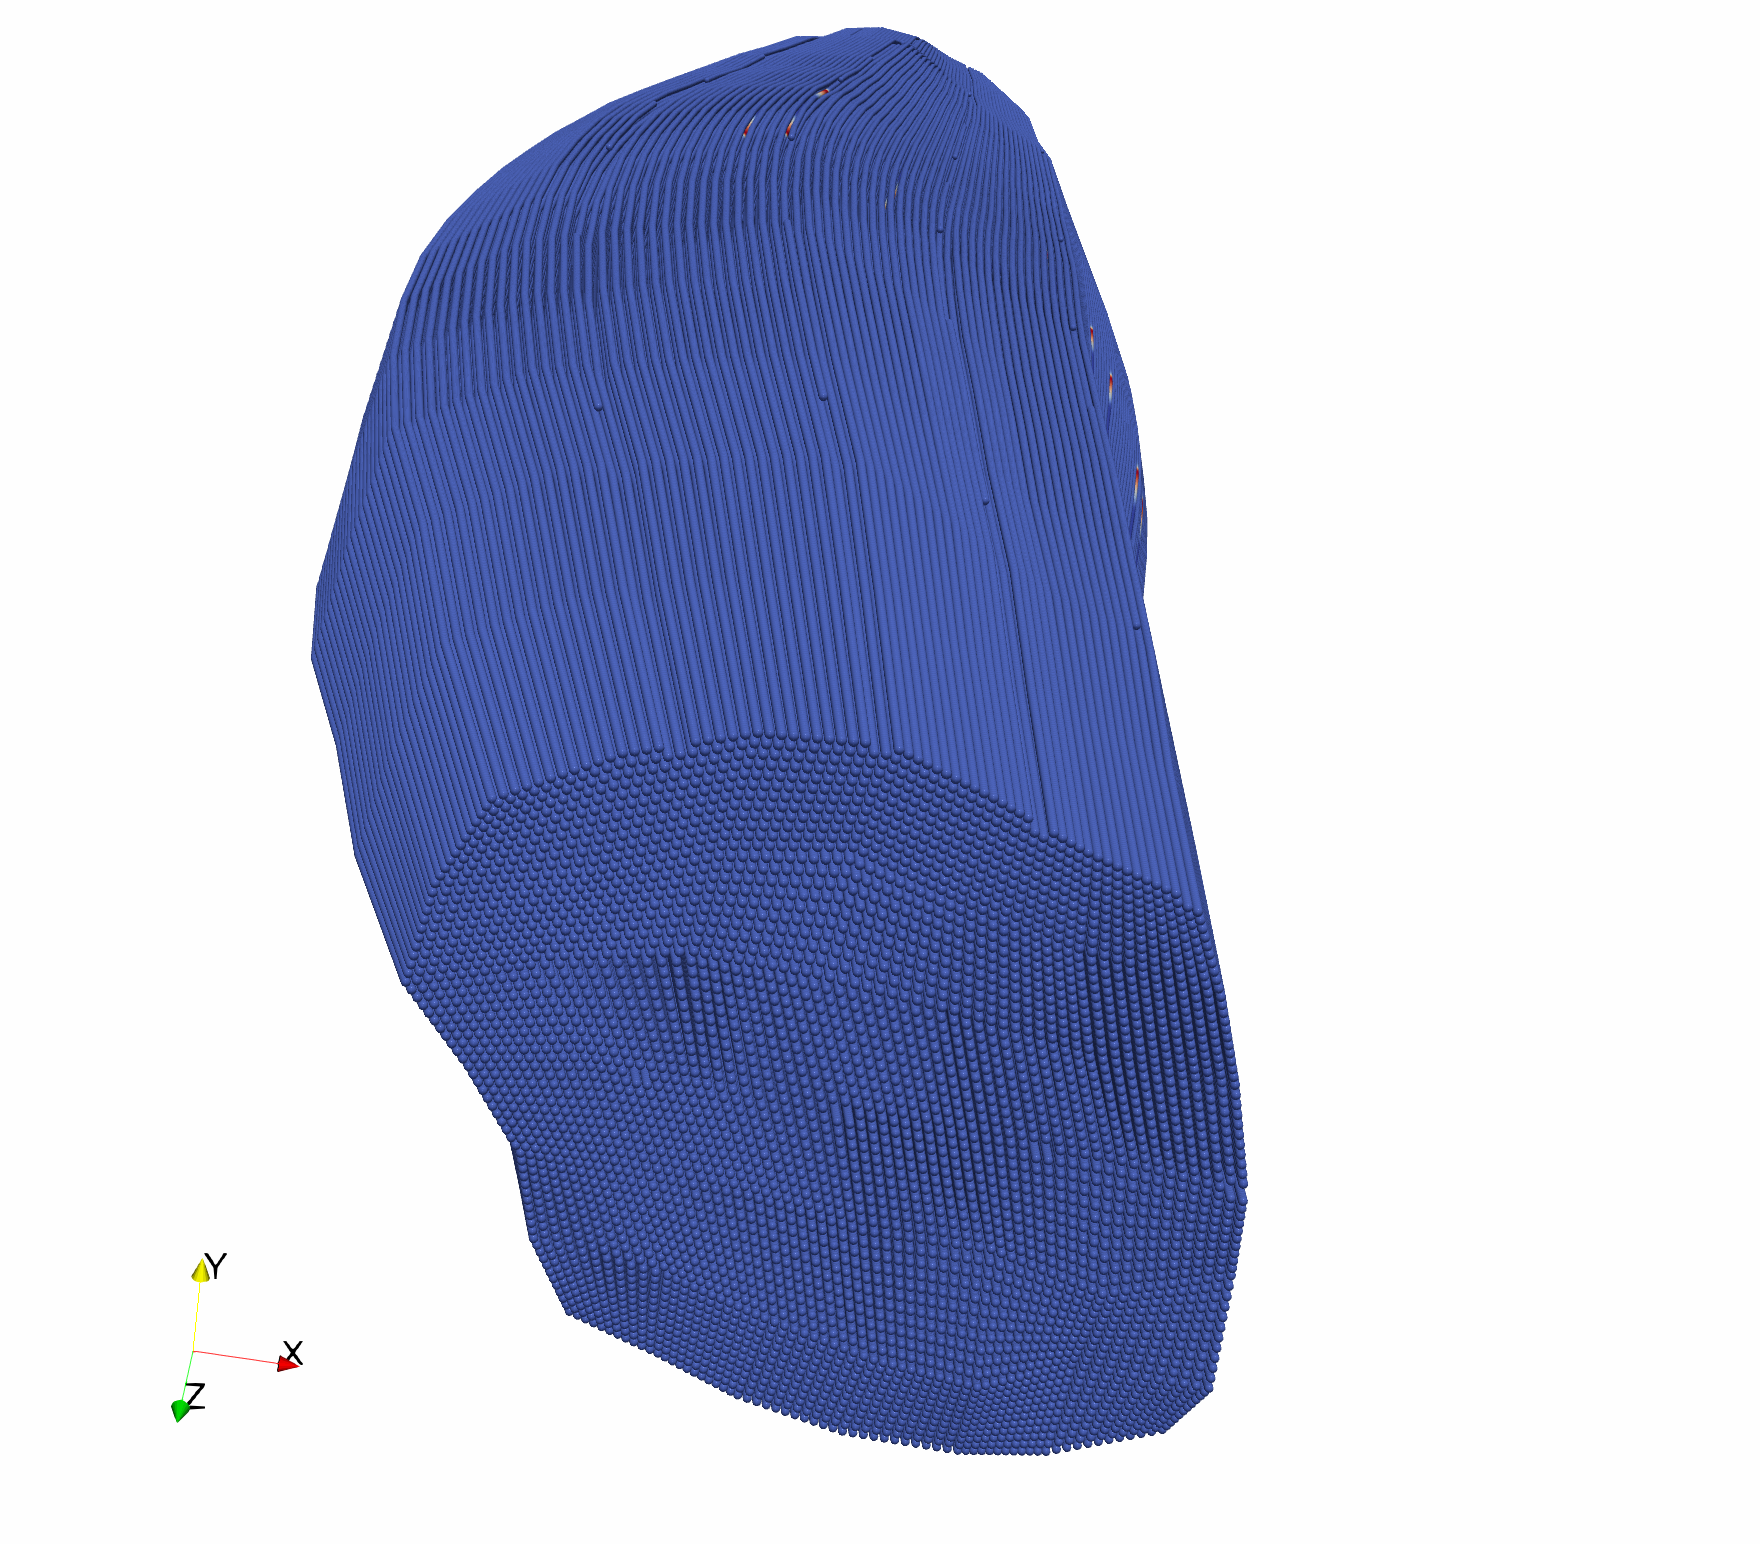
\includegraphics[height=5cm]{images/parallel_fiber_estimation/muscle_mesh_3.png}
    \caption{Grid $67 \times 67$ muscle fibers for the biceps geometry}%
    \label{fig:muscle_mesh_3}%
  \end{subfigure} 
  \,
  \begin{subfigure}[t]{0.15\textwidth}%
    \centering%
    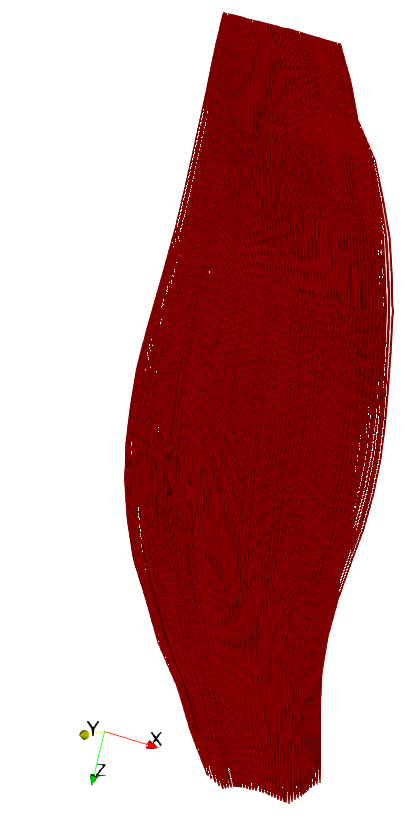
\includegraphics[height=5cm]{images/parallel_fiber_estimation/triceps_25x25.png}
    \caption{$25 \times 25$ fibers of triceps}%
    \label{fig:muscle_mesh_5}%
  \end{subfigure} 
  \hfill
  \begin{subfigure}[t]{0.55\textwidth}%
    \centering%
    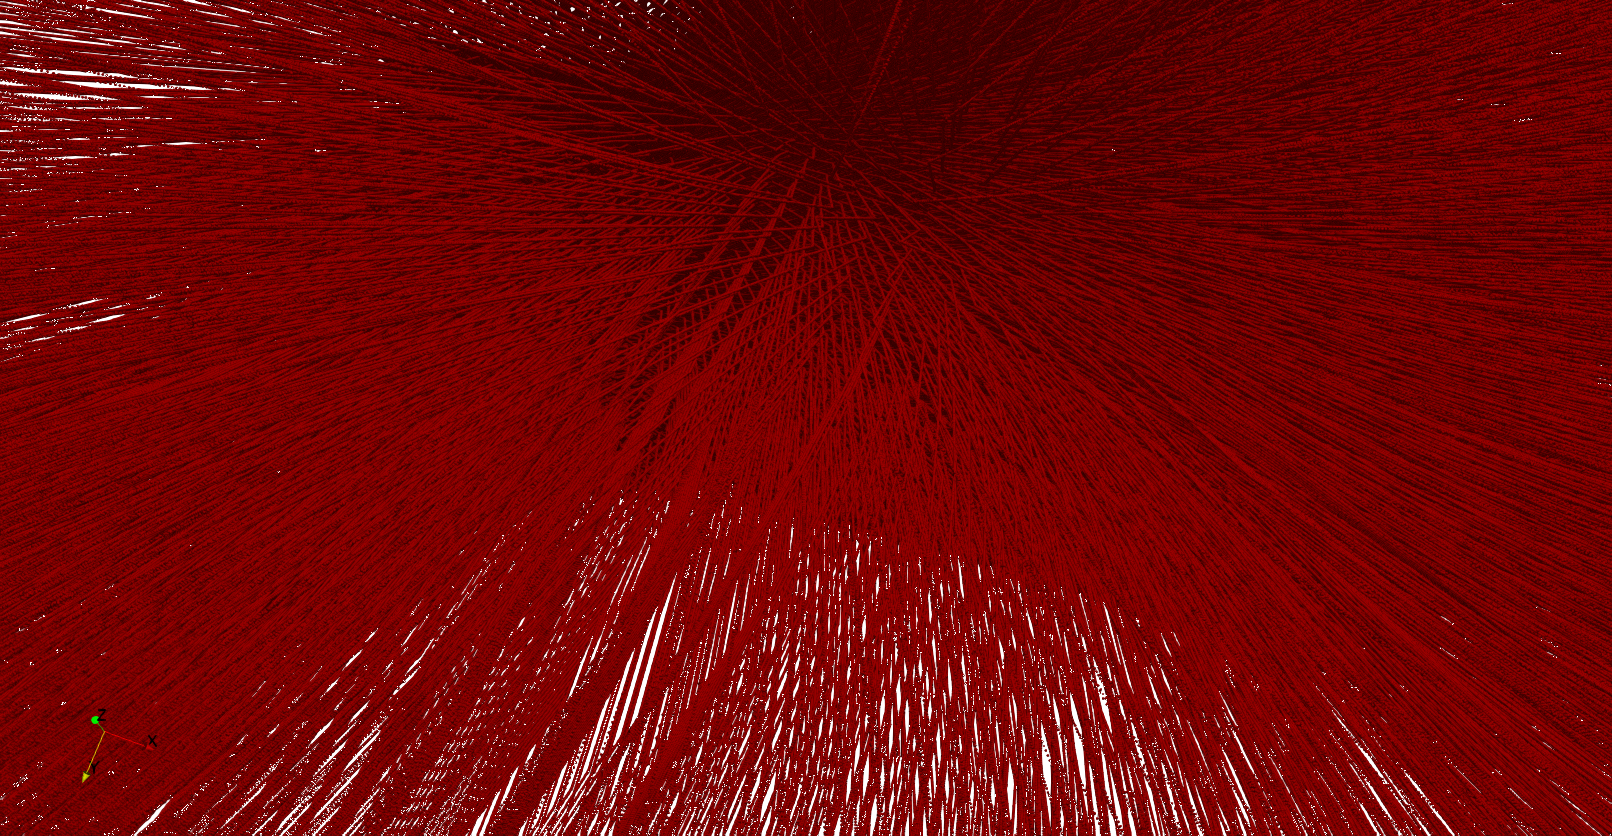
\includegraphics[width=\textwidth]{images/parallel_fiber_estimation/triceps_inside_67x67c.png}
    \caption{Grid of $67 \times 67$ fibers for the triceps geometry as seen from within the muscle. The total number of points is \num{8982489}.}%
    \label{fig:muscle_mesh_4}%
  \end{subfigure}  
   
  \caption{1D fiber meshes and corresponding 3D meshes created by \cref{alg:parallel_algorithm_1}. The biceps geometry is used in (a)-(d), the triceps geometry in (e) and (f). The fibers have 1481 nodes each in the biceps muscle and 2001 nodes each in the triceps muscle.}%
  \label{fig:muscle_meshes}%
\end{figure}%

The choices of the maximum recursion level $\ell_\text{max}$ and the fine grid parameter $m$ determine the resulting number of fibers and the file size of the binary output file. \Cref{tab:file_sizes} lists exemplary numbers of fibers and file sizes for different values of $\ell_\text{max}$ and $m$. The number $n_\text{proc}$ of required processes to reach the maximum recursion level is also listed, it depends on $\ell_\text{max}$ by $n_\text{proc}=2^{\ell_\text{max}}$. Two different numbers of fibers and corresponding file sizes are listed for every parameter combination. The two variants correspond to the two files that include respectively omit the fibers at the boundary.

The table shows that meshes with different sizes can be constructed by appropriate choices of parameters. A realistic biceps muscle contains about \num{200000} to \num{400000} muscle fibers \cite{MacDougall1984}. The table shows that constructing a mesh in this range yields a file with a size of ca. \SI{10}{\gibi\byte}. A mesh that contains \SI{1}{\percent} of the realistic number of fibers can be stored in a file with size of ca. \SI{100}{\mebi\byte}. 

The binary files to store the generated meshes are small compared to ASCII-based file formats as each point coordinate is represented by only \SI{8}{\byte}. For comparison, the ASCII-based \emph{exnode} format defined within the OpenCMISS framework uses 24 characters, i.e., \SI{24}{\byte} to store one point coordinate. Additionally, a larger memory overhead for the description of the data is needed such that \emph{exnode} files are more than three times larger than the binary files used in \opendihu{}.

The binary file format uses no compression that could further reduce the file size. The reason is that no extra effort should be needed when writing programs that parse these files. Thus, they can easily be handled by codes in different programming languages. For example, within \opendihu{} the file format is understood by various Python scripts and C++ programs.

Some numbers of fibers can be achieved with multiple, different parametrizations. \Cref{tab:file_sizes} contains such alternatives for $\ell_\text{max}$ and $m$ separated by slashes in the second and third row. For example, the combinations $(\ell_\text{max} = 0, m=3)$ as well as $(\ell_\text{max} = 2, m=0)$ both lead to a grid of $31 \times 31$ fibers (without boundary layer). However, the spatial location of the fibers in the muscle is not identical for these alternatives, as the fibers are determined by streamline tracing on differently resolved grids.
In the first case with recursion depth $\ell_\text{max} = 0$ and fine grid interpolation parameter $m=3$, many of the resulting fibers are interpolated from a coarse grid whereas in the second case with $\ell_\text{max} = 2$ and $m=0$ all fibers are key fibers and are obtained by  streamlines tracing in a fine grid.

\begin{table}
  \centering%
  \begin{tabular}{|l|l|l| r@{\,=\,}l r|rr|}
    \hline
    max.                      &fine grid     &\# proc. &  \multicolumn{2}{c}{\begin{tabular}{lrr} \# fibers && \end{tabular}}&file size \\
    level $\ell_\text{max}$   & $m$          & $n_\text{proc}$         & \multicolumn{2}{c}{\begin{tabular}{lll} &&\end{tabular}}&\\
    \hline
    0     & 0      & 1     & $9\times 9$      & \num{81} & \SI{2.7}{\mebi\byte} \\
          &        &       & $7\times 7$      & \num{49} & \SI{1.7}{\mebi\byte}\\
    0/1   & 1/0    & 1/8   & $17\times 17$    & \num{289} & \SI{9.8}{\mebi\byte}\\
          &        &       & $15\times 15$    & \num{225} & \SI{7.6}{\mebi\byte}\\
    0/1/2 & 3/1/0  & 1/8/64 & $33\times 33$    & \num{1089} & \SI{36.9}{\mebi\byte}\\
          &        &       & $31\times 31$    & \num{961} & \SI{32.6}{\mebi\byte}\\\hline
    0     & 7      & 1     & $65\times 65$    & \num{4225} & \SI{143.2}{\mebi\byte}\\
          &        &       & $63\times 63$    & \num{3969} & \SI{134.5}{\mebi\byte}\\
    2     & 7      & 64     & $257 \times 257$ & \num{66049} & \SI{2.2}{\gibi\byte}\\
          &        &       & $255 \times 255$ & \num{65025} & \SI{2.2}{\gibi\byte}\\
    2     & 15     & 64    & $513 \times 513$ & \num{263169} & \SI{8.7}{\gibi\byte}\\
          &        &       & $511 \times 511$ & \num{261121} & \SI{8.6}{\gibi\byte}\\
    \hline
  \end{tabular}
  \caption{Different parameter choices of $l_\text{max}$ and $m$ and the resulting number $n_\text{proc}$ of processes, number of fibers and file size. Some results can be achieved with different parameter combinations, e.g. both $\ell_\text{max}=0, m=1$ and $\ell_\text{max}=1, m=0$ result in $17\times 17$ fibers. These combinations are separated by slashes.}%
  \label{tab:file_sizes}%
\end{table}

\Cref{fig:different_recursion_levels} shows parts of the resulting meshes at the longitudinal center of the muscle for the two considered cases.
In \cref{fig:31x31_l0_center}, the mesh obtained with $l_\text{max}=0$ consists of a grid of traced key fibers and an interpolated finer grid of fibers. The key fiber grid  is given by the corners of the gray checkerboard pattern in the image. It can be seen that the mesh consists of patches with $4 \times 5$ or $5 \times 5$ fibers that each have equal element lengths and angles. In comparison, the mesh in \cref{fig:31x31_l2_center} that was obtained with $l_\text{max}=2$ consists only of key fibers. Here, the change in shape going from one element to its neighbors occurs more smoothly than in \cref{fig:31x31_l0_center}. This qualitatively implies a higher mesh quality.

To quantify this effect, all angles are considered that occur in an element in the $x$-$y$ plane. The mean value of all angles is $\pi/2$. The variance can be used as a measure for mesh quality. If the variance is low, this indicates similar elements and, thus, good mesh quality. 
For the present example, the variance was computed for the mesh with $31 \times 31$ fibers and \num{1481} nodes per fiber and, thus, $\num{1332000}$ 3D elements in total.
\Cref{fig:2mesh_quality} plots the variance for the three cases given in the third row of \cref{tab:file_sizes} with parameter combinations $(l_\text{max}=0,m=3)$, $(l_\text{max}=1,m=1)$ and $(l_\text{max}=2,m=0)$. Thus, the lowest bar includes the mesh shown in \cref{fig:31x31_l0_center} and the upper-most bar includes \cref{fig:31x31_l2_center}. 

It can be seen that the quality of meshes on higher recursion levels with less interpolation increases as expected.
This emphasizes the benefit of the parallel algorithm that uses finer meshes compared to the mesh used during serial execution of the algorithm.


\begin{figure}%
  \centering%
  \begin{subfigure}[t]{0.45\textwidth}%
    \centering%
    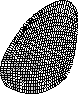
\includegraphics[width=0.9\textwidth,trim=0 0 8mm 1cm, clip]{images/parallel_fiber_estimation/31x31fibers_l0_m3_2In_dirichlet.pdf}
    \caption{Result for parameters $l_\text{max}=0, m=3$, i.e., with three interpolated fibers between every two traced fibers.}%
    \label{fig:31x31_l0_center}%
  \end{subfigure}
  \quad
  \begin{subfigure}[t]{0.45\textwidth}%
    \centering%
    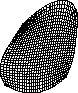
\includegraphics[width=0.9\textwidth,trim=0 0 8mm 1cm, clip]{images/parallel_fiber_estimation/31x31fibers_l2_m0_2In_dirichlet.pdf}
    \caption{Result for parameters $l_\text{max}=2, m=0$, i.e., without interpolation.}%
    \label{fig:31x31_l2_center}%
  \end{subfigure}   
   
  \caption{Comparison of generated meshes of the biceps with different maximum recursion levels $l_\text{max}$. A lower left portion of the full mesh with $31 \times 31$ fibers is shown.}%
  \label{fig:different_recursion_levels}%
\end{figure}%

\begin{figure}%
  \centering%
  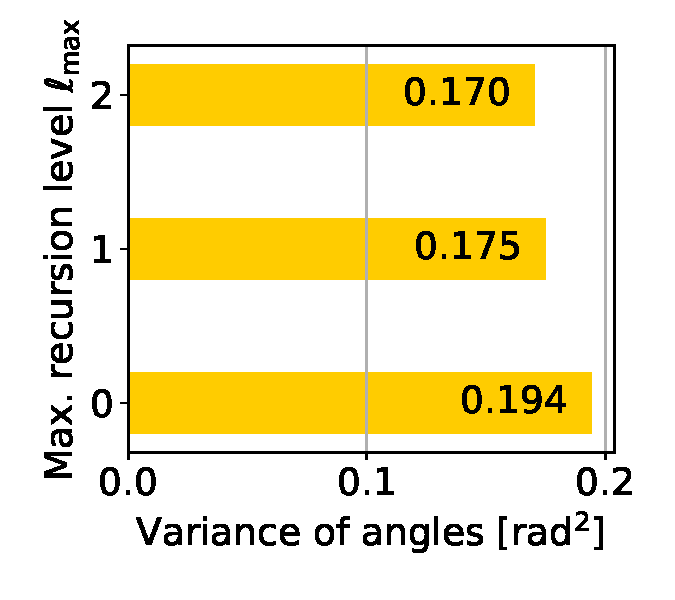
\includegraphics[height=6cm]{images/parallel_fiber_estimation/mesh_quality_recursion_level.pdf}%
  \caption{Variance of the element angles for meshes with the same number of $31 \times 31$ fibers, but created by different recursion levels $\ell_\text{max}$. The parameters correspond to the third row of \cref{tab:file_sizes}. A lower variance means better mesh quality.}%
  \label{fig:2mesh_quality}%
\end{figure}%

In addition to $l_\text{max}$ and $m$, further options exist to tune the behaviour of \cref{alg:parallel_algorithm_1}.
The number of border points in $x$ or $y$ direction as well as the number in $z$ direction can be set to different values. The number in $x$ and $y$ direction is usually set to four, the number in $z$ direction is set to 30.

Three more options are presented in the following and their effects are evaluated afterwards. First, the type of boundary conditions to the Laplace problem in \cref{eq:fiberest_laplace} can be selected among the Neumann boundary conditions given by \cref{eq:fiberest_neumann} or the Dirichlet boundary conditions given by \cref{eq:fiberest_dirichlet}.
Second, the mesh for discretizing the Laplace equation $Δp=0$ can be refined prior to the solution by increasing the number of elements per coordinate direction by the refinement factor $r \in \N$. A value of $r=1$ corresponds to no refinement, $r>1$ increases the number of 3D elements by the factor $r^3$.

%Formulations with linear or quadratic Lagrange ansatz function can be used.
Third, two options exist for computing the gradient value $\nabla p(\bfx)$ at a point $\bfx$ in the domain, which is needed for the streamline tracing.
Either, the gradient vector field is precomputed using finite differences and the nodal values of the solution field $p$.
Or the gradient value is directly interpolated at $\bfx$ in the 3D element using a linear combination of the solution values and derivatives of the ansatz functions of the element.

In the following study, the first option is indicated by the characters \say{N} or \say{D} for Neumann or Dirichlet boundary conditions, the second option is specified by an integer value for $r$ and the third option is indicated by \say{g} for the precomputed gradient field or \say{s} for using the solution values and derived ansatz functions.

For example, the scenario considered in \cref{fig:different_recursion_levels,fig:2mesh_quality} is specified as \say{D2s}, as it uses Dirichlet boundary conditions, a refinement factor of $r=2$  and the solution values to compute the gradient.

A study of all possible combinations of the three options with $r \leq 4$ was conducted.  The program was run with 8 processes. The parameters $\ell_\text{max}=1$ and $m=1$ as well as the numbers of four and 30 border points in $x$ and $z$ direction were kept constant. Thus, meshes of the same size of $31\times 31$ fibers were created by all considered variants of the algorithm.

As before, the variance of the element angles was used to rate each mesh quality. Additionally, also the variance of relative element lengths in the $x$-$y$ planes was computed, using the calculation explained in \cref{sec:mesh_generation_0_results_and_discussion}. Most scenarios yielded a value of \num{2.2e-2}. Scenarios with significantly different values were discarded, as their results contained incomplete streamlines.

The scenarios were ordered according to their mesh quality score, i.e., the variance of their element angles. \Cref{fig:3mesh_quality} plots the eight best results sorted by improving mesh quality from top to bottom.
It can be seen that all values are close together, which indicates a similar good mesh quality for all shown parameter combinations.
Nevertheless, the order shows some differences between the options. A better result was achieved if Neumann boundary conditions were used (\say{N}) compared to Dirichlet boundary conditions (\say{D}). Also, a higher refinement factor $r$ of the internal mesh was beneficial in this study. The variant without the precomputed gradient field (\say{s}) performed better than the variant with gradient field computation (\say{g}).

However, further studies with different recursion widths showed that the effect of these three options also depended on the scenario. For a higher recursion width, Dirichlet boundary conditions proved more robust in the sense that less incomplete streamlines occured. Larger refinement factors led to smaller mesh widths and in consequence to a smaller ghost layer for the streamline tracing, which always has a thickness of one element. Thus, more streamlines left their subdomain and became invalid. Therefore, e.g., a smaller value of $r$ yielded better results for $\ell_\text{max}=2$.

In summary, for the maximum recursion level $\ell_\text{max}=1$ the best parameter combination among the tested combination is \say{N4s}. For $\ell_\text{max}=2$ a good combination is \say{D2s} and should be used instead.

\begin{figure}%
  \centering%
  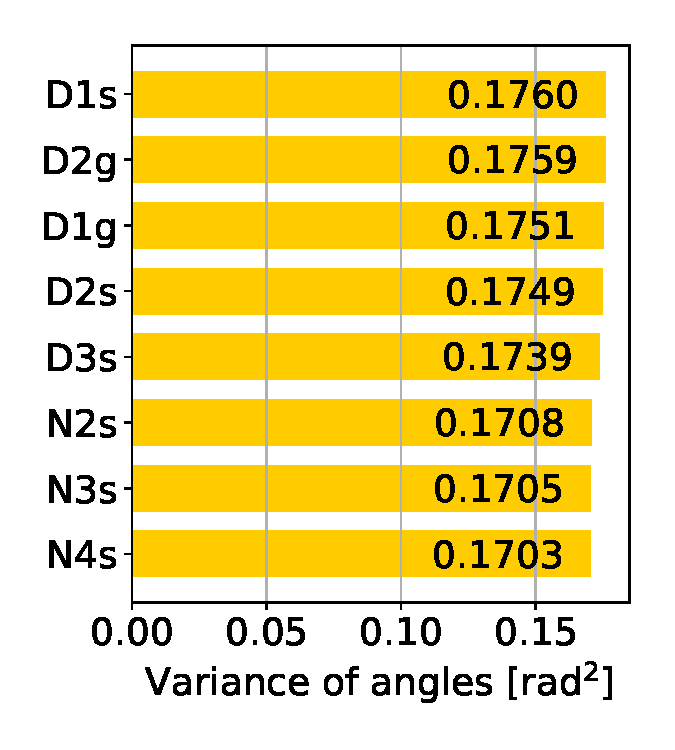
\includegraphics[height=6cm]{images/parallel_fiber_estimation/mesh_quality_options.pdf}%
  \caption{Comparison of the mesh quality that results from different options in the mesh generation algorithm. A lower variance means better mesh quality.}%
  \label{fig:3mesh_quality}%
\end{figure}%

\label{sec:repro_tendon_meshes}
\begin{reproduce}
  The parallel algorithm is implemented in the example \code{parallel_fiber_estimation}. 
  Numerous parameters can be set on the command line. After compilation, run the program as follows to get a description of all available options.
  \begin{lstlisting}[columns=fullflexible,breaklines=true,postbreak=\mbox{\textcolor{gray}{$\hookrightarrow$}\space}]
    cd $\$$OPENDIHU_HOME/examples/fiber_tracing/parallel_fiber_estimation/build_release
    ./generate ../settings_generate.py --help
  \end{lstlisting}
  Running the program without options and \code{--help} uses sensible default values. A given surface triangulation of the biceps muscle gets used by default. To compute the examples shown in this section, use and adjust the following script that runs the \code{generate} program and computes the mesh quality:
  \begin{lstlisting}[columns=fullflexible,breaklines=true,postbreak=\mbox{\textcolor{gray}{$\hookrightarrow$}\space}]
    cd $\$$OPENDIHU_HOME/examples/fiber_tracing/parallel_fiber_estimation/build_release
    ../run.sh
  \end{lstlisting}
  Computation of mesh and file sizes as shown in \cref{tab:file_sizes} can be done using the \emph{compute\_sizes.py} script.
  
  While the previously given commands are good for exploring the algorithms, generation of the meshes used for the simulation involves some more steps. Dedicated scripts exist that perform all steps and call the algorithms with the proper parameters.
  Starting from the STL file extracted from cmgui, as explained in \cref{sec:surf_extr}, the next steps are: 
  \begin{itemize}[leftmargin=1cm]
  \item[(i)] Scale the points from millimeters (used in the Visible Human dataset) to centimeters (used in the simulation), 
  \item[(ii)] remove the interior triangles, 
  \item[(iii)] translate the mesh such that the bounding box begins at $z=0$, this is needed for the programs used in the next steps, 
  \item[(iv)] create the spline surface representation as explained in \cref{sec:nurbs}, 
  \item[(v)] compile and run the \opendihu{} programs to create the binary files of the 3D mesh and the 1D fibers meshes, the algorithm in \cref{sec:parallel_algorithm} is used, 
  \item[(vi)] adjust the indexing and undo the translation in (iii), \item[(vii)] refine the created meshes of key fibers by different numbers $m$ of fine grid fibers, in total 10 different mesh sizes are created for differently refined simulations, 
  \item[(viii)] create meshes for the fat layer $\Omega_B$ ontop of the muscle surface, also in 10 different resolutions.
  \end{itemize}
  
  Two scripts are given for the biceps brachii and triceps brachii muscles. They perform all listed steps and also create intermediate output files that can be used to understand the process. Some steps are automatically skipped if the resulting output file already exists from a previous run. This is especially helpful for the removal of the interior triangles from the initial file which takes nearly a full day.
  
  A third scripts creates three meshes $\Omega_{T,i}$ for the tendons of the biceps muscle, as visualized in \cref{fig:tendon_meshes}. At the bottom, a single tendon mesh is created whereas at the top, two seperate tendons exist. The script involves numerous rotation and cropping operations of the initial surface, before the algorithm of \cref{sec:ser_alg_meshes} is executed. The three output files of the tendon meshes have the same file format as the muscle meshes. The files have the extension \emph{.bin} for \say{binary}. The script \code{examine_bin_fibers.py} can be used to debug the created binary files.
  
  The three scripts can be executed as follows:
  \begin{lstlisting}[columns=fullflexible,breaklines=true,postbreak=\mbox{\textcolor{gray}{$\hookrightarrow$}\space}]
    cd $\$$OPENDIHU_HOME/examples/electrophysiology/meshes
    ./process_meshes_biceps.sh
    ./process_meshes_triceps.sh
    ./process_meshes_tendons.sh
  \end{lstlisting}
  The output can be found in the subdirectory \code{processed_meshes}. For the total output about \SI{46}{\gibi\byte} of drive space is required.
  
\end{reproduce}

\section{Conclusion and Future Work}\label{sec:meshes_summary_and_conclusion}

This chapter presented algorithms for creating muscle meshes that are needed for multi-scale simulations of the musculoskeletal system.
For the biceps muscle, 3D meshes for tendons on both ends and the muscle were created. Additionally, 1D fibers meshes were generated that are embedded in the mesh of the muscle. The 3D mesh and the 1D meshes are aligned with each other. This facilitates data mapping between the meshes and reduces numerical errors. All generated meshes are structured, which allows an efficient parallelization.

First, an overview of available meshing software and known algorithms in the literature was given. Very little software tools were capable of generating structured meshes and none fitted our special needs. Therefore, own algorithms were developed to generate meshes starting from medical imaging data.

A workflow was presented to generate a smooth surface triangulation from imaging data. Our base data was the male dataset from the Visible Human Project. Two alternatives within this workflow were presented, where the first alternative executed automatic image segmentation based on morphological operations and the second alternative used semi-automatic segmentation tools from the Physiome project. Then, smooth NURBS surfaces were fitted to the extracted boundaries of the muscle volumes.

Next, a novel algorithm to create structured meshes from a triangulated muscle surface was presented. The algorithm used harmonic maps on 2D slices to achieve good mesh quality. A method of computing streamlines in a divergence-free vector field to estimate muscle fibers, which is established in the literature was used. It allowed to embedded 1D meshes for muscle fibers in the created 3D meshes of the muscle. Numeric experiments tested and evaluated different choices of triangulation and quadrangulation schemes for the 2D cross section and reference domains in our algorithm.

Next, a parallelized algorithm was introduced that was based on our first, serial algorithm. The algorithm used distributed memory parallelism and provided the same features as the serial algorithm, having the same formats for input and output. The difference was that it constructed a fine, partitioned mesh for streamline tracing that was distributed over all employed processes. Thus, it was possible to create finer meshes using more compute nodes. Differently resolved meshes of the biceps and triceps muscle volumes and muscle fibers were created using this algorithm. The superiority of the parallel algorithm using a higher number of processes compared to the serial execution was explained and demonstrated in a numerical experiment. Several options to fine-tune the algorithm were evaluated.

The presented algorithms and their implementation in \opendihu{} are the basis for further computations within this work. They are used to generate structured hexahedral meshes with good mesh quality. These meshes are required for efficient, parallel Finite Element simulations of various aspects of the neuromuscular system.

The presented algorithms are specialized for fusiform muscles and require the muscle geometry be oriented along one coordinate axis (the $z$ axis) in order to generate a structured mesh  that comprises planar slices that are normal to that direction.
The algorithms can also be applied to any tubular surface geometry of more complex muscles and will construct the corresponding structured 3D mesh. The generated 1D fiber meshes, however, are only valid for muscles, where the approach of streamline tracing through the solution of the Laplacian potential flow problem with boundary conditions at the bottom and top ends of the muscle can be applied.
In the literature, this approach has been successfully used for various muscles with more complex fiber architectures, such as the tibialis anterior, gluteus maximus and deltoid muscles \cite{Choi2013}. However, the locations where boundary conditions were prescribed was not always at the bottom and top ends of the muscle.

If in future work muscles with more complex layouts should be simulated, the approach could be as follows. Depending on the complexity of the outer geometry, first the presented algorithms (either \cref{alg:serial_algorithm_1,alg:serial_algorithm_2} or \cref{alg:parallel_algorithm_1}) can be used to create a structured 3D mesh. Then, a potential flow simulation can be manually setup in \opendihu{} using the 3D mesh and boundary conditions defined at proper locations. Seed points have to be defined and the streamline tracer of \opendihu{} can be used to create fiber meshes. In consequence, the resulting 1D fibers will not be aligned with the 3D mesh. Algorithmicly, this poses no problem to the simulations in \opendihu{} as the data mapping functionality can handle arbitrarily positioned meshes. However, the parallel partitioning gets more involved as the combined domain of 1D and 3D meshes has to be partitioned equally for both mesh types.

